\documentclass[a4j, twocolumn, dvipdfmx]{jsarticle}

\usepackage[a4paper, left=2.0cm, right=2.0cm, top=2.0cm, bottom=2.0cm]{geometry}
\usepackage{amsmath}   % 数式用
\usepackage{amssymb}
\usepackage[dvipdfmx]{graphicx}
\usepackage{booktabs}  % \toprule, \midrule, \bottomrule 等の表罫線用
\usepackage{titlesec}  % 見出し調整
\usepackage{enumitem}  % 箇条書きの余白調整
\usepackage{array}
\usepackage{tikz}
\usetikzlibrary{positioning}
\usepackage{algorithm}
\usepackage{algpseudocode}
\usepackage{float}
\usepackage{flushend}  % 最終ページの左右コラムの高さをそろえる
\raggedbottom
% 段組をまたぐ図表をページ上部に置きやすくする（本文から離れすぎるのを防ぐ）
\renewcommand{\topfraction}{0.9}
\renewcommand{\dbltopfraction}{0.9}
\renewcommand{\textfraction}{0.1}
\renewcommand{\floatpagefraction}{0.8}
\renewcommand{\dblfloatpagefraction}{0.8}
\setcounter{topnumber}{3}
\setcounter{dbltopnumber}{3}

% =========================================================
% 見出し設定
% =========================================================
\titleformat{\section}[block]
  {\normalfont\large\bfseries}
  {\thesection}{0.7em}{}

\titleformat{\subsection}[block]
  {\normalfont\normalsize\bfseries}
  {\thesubsection}{0.7em}{}

\titleformat{\subsubsection}[block]
  {\normalfont\normalsize\bfseries}
  {\thesubsubsection}{0.7em}{}

% titlesec は \paragraph も乗っ取るため runin 形式を明示（jsarticle での
% "Entered in horizontal mode" エラー回避）
\titleformat{\paragraph}[runin]
  {\normalfont\normalsize\bfseries}
  {\theparagraph}{0.5em}{}

% 見出し前後の余白
\titlespacing*{\section}
  {0pt}{1.5ex plus 0.5ex minus 0.2ex}{0.8ex}
\titlespacing*{\subsection}
  {0pt}{1.2ex plus 0.4ex minus 0.2ex}{0.6ex}
\titlespacing*{\paragraph}
  {0pt}{1.0ex plus 0.3ex minus 0.1ex}{0.6em}

% =========================================================
% 箇条書き設定
% =========================================================
\setlist[itemize]{topsep=4pt, itemsep=2pt, parsep=0pt, leftmargin=*}
\setlist[enumerate]{topsep=4pt, itemsep=2pt, parsep=0pt, leftmargin=1.8em}

\newcolumntype{P}[1]{>{\raggedright\arraybackslash}p{#1}}

% 指標名（周りの文章と同じ字体・太さで出すため，数式ではなく文章の書体で組む）
\newcommand{\PushRatio}{\textrm{push\_ratio}}
\newcommand{\Spread}{\textrm{spread}}
\newcommand{\Push}{\textrm{push}}

\title{
Federated Learningにおける
悪性更新の検知可能性の評価\\[0.8em]
\large
― データ分布の不均一性と攻撃のステルス性を軸として ―
}
\author{3CDA2216 笠原秀星}
\date{\today}

% 概要（タイトルの下に段組をまたいで置く）
\makeatletter
\g@addto@macro\@maketitle{%
  \begin{center}
  \begin{minipage}{0.9\textwidth}
  \small
  \textbf{概要}\quad
  Federated Learning（FL）では, 悪性クライアントが送る更新によってグローバルモデルが汚染されうる. 本研究では, 悪性更新の検知を, 集約の直前の更新ベクトルに対する二値分類として捉え, データ分布の不均一性（Non-IID度）と攻撃のステルス性の2つの観点から, 4種類の検知器の検知性能をROC-AUCにより評価した. Flowerを用いてFLを実装し, データ数を揃えたディリクレ分布によるラベルの偏りでNon-IID度を3水準に変え, 符号反転攻撃とALIE（係数 $z$ を8水準）に対して計300回の実行を行った. その結果, 検知器の優劣は攻撃によって入れ替わり, 参照方向へのコサイン距離を用いる検知器は, $z \le 1.5$ のALIEに対して悪性更新を最も正常らしいと判定した. Non-IIDは検知性能を低下させたが, その原因は正常更新のばらつきの大きさではなく, ばらつきの配分であった. また, 高次元の正常更新は平均からほぼ一定の距離に並ぶため, 平均に近い悪性更新はむしろ目立ち, 距離やノルムに基づく検知が最も難しくなったのは, 悪性更新が正常更新と同じ距離に来る付近であった. これらの結果から, 悪性更新の押し出し量と正常更新のばらつきの比で検知可能性がほぼ決まるという中心仮説は支持されず, 検知可能性は検知器が見る量の上での悪性更新の位置と, 正常更新の分布の形に依存することが示唆された.
  \end{minipage}
  \end{center}
  \vspace{0.5em}%
}
\makeatother

\begin{document}

\maketitle

% =========================================================
\section{はじめに}
\label{sec:intro}

Federated Learning（以下, FL）は, 生データを共有することなく複数のデバイスや組織が協調して機械学習モデルを学習する分散学習の枠組みである\cite{mammen2021fl}.
FLは, ユーザのプライバシー保護と機械学習の両立を可能にする技術として注目されており, スマートフォンにおける単語予測や顔認識, 音声認識技術の向上に利用されている. また, 厳格なプライバシー規制によりデータ共有が困難な医療分野や, 自動運転車におけるリアルタイムデータの活用など, 幅広い分野への応用が期待されている\cite{li2019fl}.

一方で, FLには収束性, データ分布の不均一性（Non-IID）, 通信コスト, 大規模環境への適用, モデル集約手法など, さまざまな課題が存在する\cite{ma2020privacy}. 特に, FLでは多数の参加者が学習に関与するため, 悪意のあるクライアントによる攻撃への耐性を確保することが重要な研究課題となっている. 医療データや個人情報などの機密性の高いデータを扱う応用が想定されることから, 安全かつ信頼性の高い学習環境の実現が求められている.

FLに対する代表的な攻撃としてPoisoning Attackが挙げられる. Poisoning Attackは大きくData Poisoning AttackとModel Poisoning Attackの2種類に分類される. Data Poisoning Attackは学習データそのものを改ざんする攻撃であり, ラベル反転攻撃やBackdoor Attackなどが含まれる. 一方, Model Poisoning Attackはクライアントがサーバへ送信するモデル更新や勾配情報を改ざんする攻撃であり, 勾配操作や最適化手法を利用した攻撃などが提案されている.

これらの攻撃に対する防御手法としては, 異常検知, Robust Aggregation, 摂動機構の3つに大別される. 異常検知にはコサイン類似度やクラスタリング, スコアベース手法などが用いられる. また, Robust AggregationにはKrum, Trimmed Mean, Median, Bulyanなどの集約手法が提案されている. さらに, 摂動機構としては差分プライバシーを利用した手法が広く研究されている\cite{sagar2023survey}.

本研究では, これらの中でもModel Poisoning Attackに着目する. Data Poisoning Attackに関してはこれまで多くの研究が行われており, 攻撃に対してロバストな集約手法や検知手法が多数提案されている. 一方で, Model Poisoning Attackは学習データではなくモデル更新そのものを改ざんするため, サーバ側から攻撃を識別することが困難であり, より深刻な脅威となる. そのため, Model Poisoning Attackに対する防御は依然として重要な研究課題とされている\cite{sagar2023survey}.

さらに, 防御を回避するよう設計された攻撃も提案されている. Fangら\cite{fang2020local}はRobust Aggregationの特性を突く攻撃を, Baruchら\cite{baruch2019little}は正常更新のばらつきの範囲内に収まるよう悪性更新を作る攻撃ALIEを示した. このようなステルス攻撃は, 悪性更新を正常更新の中に紛れ込ませることで防御をすり抜ける.

攻撃と防御の攻防は, 各ラウンドでサーバが集約を行う直前の更新ベクトル空間で生じている. そこで本研究では, 防御を, 悪性更新と正常更新を識別する二値分類（異常検知）問題として捉え, モデルの最終精度ではなく更新ベクトルレベルの検知性能で評価する. 本研究では, データ分布の不均一性（Non-IID度）と攻撃のステルス性を2軸に, 集約手法に依存しない代表的な検知器が悪性更新をどこまで見分けられるか, そしてどの条件で検知が破綻するかを明らかにする.

検知性能を集約手法と切り離して評価するのは, 検知が集約とは独立の前段として用いられるためである. 検知で悪性と判定された更新は, 集約の前に除外したり重みを下げたりでき, FedAvgにもRobust Aggregationにも組み合わせられる. 特にALIEのようなステルス攻撃は, Trimmed MeanやKrumなどのRobust Aggregationを回避するよう設計されており, 原論文では外れ値を除外しない単純な平均よりも, むしろRobust Aggregationを用いた場合に精度を大きく低下させた\cite{baruch2019little}. そのため, 集約の前段で悪性更新を見分けられるかどうかは, Robust Aggregationを用いる場合にこそ重要になる. 本研究では, 集約手法の影響を受けずに更新ベクトルそのものの見分けやすさを測るため, 集約には最も単純なFedAvgを用い, 検知結果は集約に用いない.

本論文の構成は次のとおりである. 第\ref{sec:prelim}章でFL, Poisoning Attack, 防御手法, および検知性能の評価指標について述べ, 第\ref{sec:related}章で関連研究を整理する. 第\ref{sec:rq}章で研究の問いと仮説を, 第\ref{sec:threat}章で脅威モデルを, 第\ref{sec:framework}章で評価枠組みを示す. 第\ref{sec:experiment}章で実験の設定を述べ, 第\ref{sec:results}章でその結果を, 第\ref{sec:discussion}章で考察を示す. 最後に第\ref{sec:conclusion}章で本論文をまとめる.

% =========================================================

\section{基礎知識}
\label{sec:prelim}

\subsection{Federated Learning}
第\ref{sec:intro}章で述べたように, FLは生データを共有することなく複数のデバイスや組織が協調して機械学習モデルを学習する分散学習の枠組みである\cite{mammen2021fl}. FLにおける代表的な集約アルゴリズムとして, McMahanら\cite{mcmahan2017fedavg}が提案したFederated Averaging（以下, FedAvg）がある. 本研究でもサーバ側の集約にはFedAvgを用いる.

\subsubsection{FedAvg}
\begin{table}[t]
\centering
\caption{FedAvgで用いる主な記号}
\begin{tabular}{ll}
\hline
記号 & 意味 \\
\hline
$K$ & 全クライアント数 \\
$C$ & 各ラウンドで参加する割合 \\
$S_t$ & ラウンド$t$で選択されたクライアント集合 \\
$w_t$ & グローバルモデル \\
$w_{t+1}^k$ & クライアント$k$が更新したモデル \\
$n_k$ & クライアント$k$のデータ数 \\
$E$ & ローカル学習のエポック数 \\
$b$ & ミニバッチサイズ \\
$\eta$ & 学習率 \\
\hline
\end{tabular}
\label{tab:fedavg_symbol}
\end{table}
\begin{algorithm}[t]
\caption{Federated Averaging (FedAvg)}
\label{alg:fedavg}
\begin{algorithmic}[1]
\State \textbf{Server executes:}
\State Initialize $w_0$
\For{each round $t = 1,2,\ldots$}
    \State $m \leftarrow \max(C \cdot K, 1)$
    \State $S_t \leftarrow$ random set of $m$ clients
    \ForAll{$k \in S_t$ in parallel}
        \State $w_{t+1}^{k} \leftarrow \mathrm{ClientUpdate}(k,w_t)$
    \EndFor
    \State $
    w_{t+1}
    \leftarrow
    \sum_{k \in S_t}
    \frac{n_k}{n_t}
    w_{t+1}^{k}
    $
\EndFor
\Statex
\State \textbf{ClientUpdate}$(k,w)$
\State Split $P_k$ into mini-batches of size $b$
\For{$i=1$ to $E$}
    \For{each mini-batch $\xi$}
        \State $
        w \leftarrow
        w-\eta\nabla\ell(w;\xi)
        $
    \EndFor
\EndFor
\State \Return $w$ to server
\end{algorithmic}
\end{algorithm}
アルゴリズム\ref{alg:fedavg}にFedAvgの処理手順を示す.

まず, サーバはグローバルモデル $w_0$ を初期化する.
その後, 各通信ラウンド $t$ において, 全クライアント数 $K$ のうち割合 $C$ に応じた $m$ 個のクライアントをランダムに選択する.
選択されたクライアント集合を $S_t$ とする.

選択された各クライアントは, サーバから受け取ったグローバルモデル $w_t$ を用いてローカル学習を実施する.
各クライアントは自身が保有するデータ集合 $P_k$ をサイズ $b$ のミニバッチに分割し, エポック数 $E$ 回の学習を行う.
モデル更新には確率的勾配降下法（SGD）を用い, 学習率を $\eta$ とすると, 各ミニバッチ $\xi$ に対して次式によりパラメータを更新する.

\begin{equation}
w \leftarrow w-\eta\nabla \ell(w;\xi)
\end{equation}

ここで, $\ell(w;\xi)$ はミニバッチ $\xi$ に対する損失関数であり, $\nabla \ell(w;\xi)$ はその勾配を表す.

ローカル学習終了後, 各クライアントは更新後のモデル $w_{t+1}^{k}$ をサーバへ送信する.
サーバは受信したモデルを, 各クライアントの保有データ数 $n_k$ に応じて重み付け平均することで新たなグローバルモデル $w_{t+1}$ を生成する.

\begin{equation}
w_{t+1}
=
\sum_{k \in S_t}
\frac{n_k}{n_t}
w_{t+1}^{k},
\qquad
n_t=\sum_{k\in S_t}n_k
\end{equation}

この処理を複数ラウンド繰り返すことで, 生データを共有することなくグローバルモデルを学習する.

\subsection{データ分布の不均一性（Non-IID）}
\label{sec:noniid}

FLでは, 各クライアントが保有するデータは, 利用者や組織ごとの違いを反映して互いに異なる分布を持つことが多い. 全クライアントのデータが同一の分布から独立に得られている場合をIID（independent and identically distributed）と呼び, そうでない場合をNon-IIDと呼ぶ. Non-IID環境では, 各クライアントのローカル学習が異なる方向へ進むため, モデル更新がクライアント間でばらつく.

Non-IIDにはいくつかの種類がある. NIID-Bench\cite{li2022federated}は, FLの実験で扱うNon-IIDを次の3つに整理している.
\begin{itemize}
  \item \textbf{ラベル分布の偏り}（label distribution skew）: クラスの比率がクライアントごとに異なる.
  \item \textbf{特徴分布の偏り}（feature distribution skew）: 入力の分布がクライアントごとに異なる. 例えば, 同じ数字でも筆跡が異なる場合がこれにあたる.
  \item \textbf{データ数の偏り}（quantity skew）: データの分布は同じでも, 保有するデータ数がクライアントごとに異なる.
\end{itemize}
これらは同時に生じうる. 本研究で扱うNon-IIDがどの種類にあたるかは, \ref{sec:data-noniid}節で述べる.

\subsection{Data Poisoning Attack}

Data Poisoning Attackは, 攻撃者が学習データそのものを改ざんし, グローバルモデルの性能低下や誤動作を引き起こす攻撃である. FLでは, 各クライアントが保有するローカルデータや学習過程をサーバが直接確認できないため, 悪意のあるクライアントが改ざんしたデータを用いて学習を行うことで, モデルに悪影響を与えることが可能である\cite{sagar2023survey}.

Data Poisoning Attackは, Label Flipping Attack, Poisoning Sample Attack, Backdoor Attackなどに分類される. Label Flipping Attackは, 学習データのラベルを意図的に別のラベルへ変更する攻撃である. 一方, Backdoor Attackは, 特定のトリガを含む入力に対してのみ誤分類を引き起こす攻撃であり, 通常の入力に対する性能を維持したままトリガ入力のみを誤らせるためステルス性が高い.

Data Poisoning Attackは実装が比較的容易である一方, 異常なデータ分布やラベルの偏りを利用した検知手法によって防御できる場合がある. そのため近年では, 学習データではなくモデル更新そのものを改ざんするModel Poisoning Attackに関する研究が盛んに行われている\cite{sagar2023survey,xie2020dba,nguyen2022flame}.

\subsection{Model Poisoning Attack}

Model Poisoning Attackは, 悪意のあるクライアントがサーバへ送信するモデル更新や勾配情報を改ざんし, グローバルモデルの性能低下や誤動作を引き起こす攻撃である. Data Poisoning Attackが学習データそのものを改ざんするのに対し, Model Poisoning Attackは学習後のモデルパラメータを直接操作する点に特徴がある. そのため, サーバ側から攻撃の有無を判断することが困難であり, FLにおける深刻な脅威の一つとして注目されている\cite{sagar2023survey}.

Model Poisoning Attackは, 勾配の符号反転やランダム勾配の挿入といった単純な操作から, 攻撃効果を最大化するようにモデル更新を最適化する手法までを含む. 特に後者は, 正常なモデル更新との差を小さく保ちながら攻撃目的を達成することで, 異常検知や防御機構による検出を回避しようとする\cite{bagdasaryan2020model}. Fangら\cite{fang2020local}のAdaptive Model Poisoning Attackや, min-max攻撃\cite{shejwalkar2021manipulating}はこの系譜に位置づけられる.

\subsection{防御手法}

前述のとおり, Poisoning Attackに対する防御は異常検知, Robust Aggregation, 摂動機構の3つに大別される\cite{sagar2023survey}. 本研究はこのうち異常検知を主対象とし, Robust Aggregationは比較・背景として扱う.

\subsubsection{Robust Aggregation}
Robust Aggregationは, 悪意のあるクライアントによる異常なモデル更新の影響を軽減することを目的とした集約手法である. 従来のFedAvgでは各クライアントの更新を重み付き平均するため, 極端な更新を送る悪性クライアントの影響を受けやすい. Byzantine Fault Toleranceの考え方を取り入れた代表的な手法として, Median, Trimmed Mean, Krum, Bulyanがある. Median\cite{yin2018byzantine}は座標ごとに中央値を採用することで, 極端な値の影響を抑える. Trimmed Mean\cite{yin2018byzantine}は座標ごとに上下 $\beta$ 個の値を除外してから平均をとる. Krum\cite{blanchard2017krum}は各更新と他の更新との距離を計算し, 近傍が最も密な1つの更新を採用する. Bulyan\cite{elmhamdi2018hidden}はKrumで候補を絞り込んだうえでTrimmed Meanを適用する手法であり, 高いByzantine耐性を持つ一方で, クライアント数 $n$ と悪性クライアント数 $f$ に対して $n \geq 4f+3$ を必要とする.

\subsubsection{異常検知}
異常検知は, サーバが受け取った各クライアントの更新ベクトルを調べ, 正常な更新の分布から外れたものを悪性候補として検出・除外・重み下げする防御である. 代表的な手掛かりとして, (i)更新ノルムの大きさ\cite{nguyen2022flame}, (ii)他クライアントや集約基準方向とのコサイン類似度\cite{nguyen2022flame}, (iii)更新ベクトル集合のクラスタリング\cite{shen2016auror}, (iv)主成分・特異値分解によるスペクトル外れ値\cite{tran2018spectral,shejwalkar2021manipulating} がある. 本研究ではこれらを, 集約手法に依存しない汎用検知器として第\ref{sec:framework}章で定式化する.

\subsection{検知性能の評価指標}
\label{sec:roc-auc}

異常検知器は各サンプルに異常スコア $s$（大きいほど異常らしい）を与え, 閾値 $\tau$ を用いて $s \geq \tau$ のサンプルを異常（陽性）と判定する. 悪性を陽性, 正常を陰性とすると, 判定結果は真陽性（TP）, 偽陽性（FP）, 真陰性（TN）, 偽陰性（FN）の4通りに分けられ, 次の2つの率が定義される.
\begin{equation}
\mathrm{TPR} = \frac{\mathrm{TP}}{\mathrm{TP}+\mathrm{FN}}, \qquad
\mathrm{FPR} = \frac{\mathrm{FP}}{\mathrm{FP}+\mathrm{TN}}
\end{equation}
TPR（真陽性率, 再現率）は悪性のうち正しく検出できた割合, FPR（偽陽性率）は正常のうち誤って悪性と判定した割合である.

\paragraph{ROC曲線とAUC}
TPRとFPRはいずれも閾値 $\tau$ に依存し, $\tau$ を下げるほど両者は増加する. $\tau$ を $+\infty$ から $-\infty$ まで動かしたときの点 $(\mathrm{FPR}, \mathrm{TPR})$ の軌跡をROC（Receiver Operating Characteristic）曲線と呼び, その下側の面積をROC-AUC（Area Under the Curve, 以下AUC）と呼ぶ\cite{fawcett2006roc}. AUCは特定の閾値を選ばずに, スコアによる順位付けそのものの良さを $[0,1]$ の1つの値で表す.

AUCは次の確率的な解釈を持つ\cite{hanley1982meaning}. 陽性集合を $M$, 陰性集合を $B$ とすると,
\begin{equation}
\mathrm{AUC}
= \frac{1}{|M|\,|B|}\sum_{i \in M}\sum_{j \in B}
\Bigl( \mathbf{1}[s_i > s_j] + \tfrac{1}{2}\,\mathbf{1}[s_i = s_j] \Bigr)
\label{eq:auc}
\end{equation}
であり, これは「ランダムに選んだ悪性サンプルのスコアが, ランダムに選んだ正常サンプルのスコアを上回る確率」に等しい. したがって, $\mathrm{AUC}=1$ はすべての悪性が正常より上位に並ぶ完全な分離, $\mathrm{AUC}=0.5$ はランダムな順位付けと同等であることを表す. $\mathrm{AUC}<0.5$ は検知器が悪性を正常より「正常らしい」と評価していることを意味し, 正常更新に紛れ込むよう設計されたステルス攻撃に対しては起こりうる.

\paragraph{閾値非依存指標を用いる理由}
正解率（accuracy）やF1値は閾値を1つ固定して算出するため, 値が閾値の選び方に左右される. また悪性が少数派の不均衡な設定では, すべてを正常と判定するだけで正解率が高くなってしまう. AUCはTPRとFPRをそれぞれ陽性・陰性の内部で正規化するためクラス比の影響を受けにくく, 検知器が悪性と正常を分離できているかを評価するのに適している.

\paragraph{小標本での注意}
式(\ref{eq:auc})が示すように, AUCは悪性と正常のペア $|M|\,|B|$ 組の比較で決まる. 1ラウンドあたりのクライアント数が少ない場合, AUCが取りうる値は離散的になり（例えば $|M|=4$, $|B|=16$ では $1/64$ 刻み）, 1組の順位の入れ替わりで値が変動する. そのため本研究では, ラウンド単位のAUCを複数ラウンド・複数試行にわたって集計して評価する.

% =========================================================
\section{関連研究}
\label{sec:related}

Sagarらは, FLにおけるPoisoning Attackおよび防御手法に関する包括的なサーベイを行っている. 彼らは攻撃をData Poisoning AttackとModel Poisoning Attackに分類し, 防御手法についてもRobust Aggregationや異常検知手法などの観点から体系的に整理している\cite{sagar2023survey}.

Fangらは, Byzantine-robustなFLに対するLocal Model Poisoning Attackを提案した. 攻撃を最適化問題として定式化することで, Krum, Bulyan, Median, Trimmed MeanといったByzantine-robust Aggregation手法に対しても有効な攻撃を実現し, 既存の防御手法が十分ではないことを示した\cite{fang2020local}.

Robust Aggregationの基礎としては, BlanchardらのKrum\cite{blanchard2017krum}, Yinらの座標ごとMedian/Trimmed Mean\cite{yin2018byzantine}, El MhamdiらのBulyan\cite{elmhamdi2018hidden} がある. これらは一定割合以下のByzantineクライアントに対する理論的保証を与えるが, いずれも「正常更新が互いに近い」ことを暗に仮定しており, Non-IID環境では保証が弱まる.

Baruchらは, 正常更新の座標ごとの標準偏差の範囲内に収まる小さな摂動を悪性クライアント全員が協調して送る``A Little Is Enough''（ALIE）攻撃を提案し, Trimmed Mean, Krum, Bulyanを回避できることを示した\cite{baruch2019little}. Shejwalkarらは, 集約手法非依存のmin-max/min-sum攻撃と, 特異値分解に基づく検知（Divide-and-Conquer）を提案した\cite{shejwalkar2021manipulating}.

検知型防御としては, コサイン距離のクラスタリングと重みクリッピングを組み合わせるFLAME\cite{nguyen2022flame}がある.

データ分布の不均一性の扱いとしては, Hsuらのディリクレ分布によるラベル分割\cite{hsu2019measuring} が標準的であり, NIID-Bench\cite{li2022federated} が各種分割方式を体系的に比較している.

本研究に特に近い2つの先行研究がある. Liらは, FedSGD/FedAvg上で8種のRobust Aggregation手法と5種のByzantine攻撃（ALIE等を含む）をIID/Non-IID双方で比較する実験的研究を行い, Non-IIDデータでは全手法の頑健性が大きく低下し, 一部は悪性クライアントが皆無でも性能が悪化することを示した\cite{li2023experimental}. ただし彼らの評価指標は最終精度であり, 学習の過程で頑健性がどう変化するかは扱っていない. また, Wangらは, コサイン類似度・$L_2$ノルム・ユークリッド距離といった類似度指標が高次元パラメータ空間では, パラメータの値が大きく異なっていても類似と評価されうるという欠点を持つことを示し, この欠点を突く攻撃Fakerを提案した\cite{wang2023trust}. この結果は, コサイン距離に基づく検知器（本研究のD2に相当）が攻撃によって欺かれうることを示している.

これらの研究の多くは, 最終精度や攻撃成功率によって評価するか, 検知性能を単一のNon-IID水準でのみ報告している. これに対し本研究は, Non-IID度と攻撃のステルス性の両方を変化させ, 更新ベクトルレベルの検知性能を最終精度とは切り離して評価する. 本研究の特徴は次の3つである. 第一に, 各ラウンドの更新ベクトルに対して測定できるROC-AUCを主な評価指標とし, 学習の段階によって検知性能がどう変化するかを追う. 第二に, Liら\cite{li2023experimental}が報告したNon-IID環境での頑健性の低下を, 正常更新のばらつき（\PushRatio{}）と正常更新の分布の形の観点から説明することを試み, この説明が成り立つ条件と成り立たない条件を示す. 第三に, Wangら\cite{wang2023trust}が指摘した類似度に基づく検知の限界が, 既存のステルス攻撃であるALIEに対してどの条件で現れるかを実験的に調べる. なお, 本研究はNon-IID環境に最適化された新しい攻撃を提案するものではなく, 検知性能と正常更新のばらつきの関係を分析するものである.

% =========================================================
\section{研究の問いと仮説}
\label{sec:rq}

\subsection{研究の問い}

本研究では, 次の3つの問いを明らかにする. 第一に, FLにおける悪性更新は更新ベクトルレベルの異常検知でどの程度見分けられるか, また検知性能は集約手法に依存しない代表的な検知器の間でどう異なるか. 第二に, データ分布の不均一性（Non-IID度）は検知性能をどう低下させるか, またその低下は正常更新のばらつきの増大によって説明できるか. 第三に, 攻撃のステルス性, すなわち悪性更新を正常クラスタ内に収める度合いは検知性能をどう左右するか, また検知が破綻する境界はどこにあるか.

\subsection{中心仮説}

\begin{quote}
悪性更新が検知可能かどうかは, 悪性更新の押し出し量が正常クライアント間のばらつきを超えているかでほぼ決まる. Non-IIDは正常更新のばらつきを増大させるため, 攻撃を正常な多様性の中へ紛れ込ませ, 検知性能を低下させる.
\end{quote}

この仮説を検証するための説明変数として, 正常クラスタの広がり \Spread{}, 悪性更新の押し出し距離 \Push{}, およびその比 \PushRatio{}（\ref{sec:metrics}節で定義）を導入する. 仮説が正しければ, 検知性能（ROC-AUC）は \PushRatio{} が $1$ を下回る領域で急落し, Non-IID度が強いほど同じ攻撃強度でも \PushRatio{} が小さくなる, という関係が観測されるはずである. ただし, \ref{sec:attacks}節で示すとおり, ALIE（A2）では \PushRatio{} が構成上ほぼ攻撃の係数 $z$ に等しく, Non-IID度によって変化しない. このため, \PushRatio{} とAUCの観測上の関係は符号反転攻撃（A1）で調べる. 一方, A2では $z$ を選ぶことで \PushRatio{} を直接設定できる. そこでA2は, \PushRatio{} を $1$ の上下に動かしたときにAUCがどう変わるかを調べる条件として用いるとともに, \PushRatio{} をほぼ一定に保ったままNon-IID度だけを変える条件としても用いる（\ref{sec:attacks}節）.

% =========================================================
\section{脅威モデル}
\label{sec:threat}

本研究では, 攻撃者と防御者について次の脅威モデルを仮定する. 攻撃者はfull knowledgeを持つものとする. すなわち, 悪性クライアントは各ラウンドで正常クライアントの更新を参照でき, 互いに結託できる. 本実験では, この攻撃者をサーバ側で模擬する. 悪性クライアントの集合は全ラウンドを通じて固定し, その割合は $f/n \le 0.3$ を想定し, 本実験では $f/n = 0.2$ とする.

防御者はサーバ側に位置し, 全クライアントの更新ベクトルを観測できるが, クリーンなデータは持たない. したがって, FLTrust\cite{cao2021fltrust}のように, サーバが少量のクリーンなデータを持ち, それを信頼の基準とする防御は対象外とする. また, どのクライアントが悪性かという正解ラベルは評価にのみ用い, 検知器には一切与えない.

この脅威モデルは攻撃者に有利な楽観的設定である. Shejwalkarら\cite{shejwalkar2022back}は現実的な制約下ではpoisoningの脅威が限定的であると論じているが, 本研究は「検知性能の上限」を評価するものとして位置づける.

% =========================================================
\section{評価枠組み}
\label{sec:framework}

\subsection{記法}

通信ラウンド $t$ において, 参加クライアント $i \in \{1,\dots,n\}$ のモデル更新ベクトルを $g_i = w_i - w_{\text{global}}$ とする. 正常クライアントの添字集合を $B$, 悪性クライアントの添字集合を $M$（$|M| = f$）とし, $\bar{g}_B = \frac{1}{|B|}\sum_{i \in B} g_i$ を正常更新の平均とする. 本研究では毎ラウンド全クライアントが参加するため, 参加クライアント数 $n$ は表\ref{tab:fedavg_symbol}の $K$ に等しい（$C=1$）. なお, 表\ref{tab:fedavg_symbol}の $n_k$ はクライアント $k$ のデータ数であり, クライアント数 $n$ とは異なる.

\subsection{検知器}
\label{sec:detectors}

本研究では, 集約手法に依存しない汎用的な4種の検知器D1--D4を用いる. いずれの検知器も, 各クライアント $i$ に異常スコア $s_i$（大きいほど悪性らしい）を与える.

\paragraph{D1: ノルム偏差}
\begin{equation}
s_i = \left|\; \|g_i\|_2 - \operatorname*{median}_{j}\|g_j\|_2 \;\right|
\end{equation}
偶数台のクライアントでは, 中央値を挟む2台のスコアは定義上等しくなるため, 数値誤差によらず同値として扱う. D1は最も単純な検知器であり, ノルムを大きく変える攻撃（スケーリングやランダムノイズ）の検知には有効だが, ステルス攻撃には弱いと予想される. FLAME\cite{nguyen2022flame}などの重みクリッピング系の防御に対応する.

\paragraph{D2: 参照方向へのコサイン距離}
座標ごとの中央値 $r = \operatorname{median}(g_1,\dots,g_n)$ を参照方向とし,
\begin{equation}
s_i = 1 - \frac{g_i \cdot r}{\|g_i\|_2\,\|r\|_2}.
\end{equation}
D2は更新の向きの異常を捉える検知器であり, FLAME\cite{nguyen2022flame}の考え方に対応する.

\paragraph{D3: 2クラスタリング}
各更新のノルム $\|g_i\|_2$, D2スコア, および第1・第2主成分への射影の4つを特徴量 $\phi_i$ とし, 特徴量ごとに標準化したうえで $k$-means（$k=2$）を適用し, 大きい方のクラスタを正常とみなして, その重心までの距離をスコアとする. 初期中心は全ての2点の組を試し, クラスタ内平方和が最小となる分割を採用する. Auror\cite{shen2016auror}の考え方に対応する.

\paragraph{D4: スペクトル残差}
各更新を中心化した $\tilde{g}_i = g_i - \frac{1}{n}\sum_{k=1}^{n} g_k$ を並べた行列 $\tilde{G} = [\tilde{g}_1;\dots;\tilde{g}_n]$ の第1右特異ベクトル $v$ を求め,
\begin{equation}
s_i = (\tilde{g}_i \cdot v)^2
\end{equation}
とする. D4はSpectral Signatures\cite{tran2018spectral}やDivide-and-Conquer\cite{shejwalkar2021manipulating}の考え方に対応する.

\subsection{攻撃}
\label{sec:attacks}

\paragraph{A1: 符号反転攻撃}
\begin{equation}
g_i^{\text{mal}} = -\,g_i \qquad (i \in M)
\end{equation}
各悪性クライアントは自身のローカルデータで正常に学習した更新 $g_i$ の符号を反転して送る. 向きは自身の正常更新と正反対になる一方, ノルムは変わらない. A1は, 向きに基づく検知器であれば容易に検知できるはずの粗い攻撃であり, ベースラインとして用いる.

\paragraph{A2: ALIE}
本研究では, Baruchら\cite{baruch2019little}が提案したALIE（A Little Is Enough）の, 平均および標準偏差に基づく更新生成則を用いる. 攻撃者は正常更新の座標ごとの平均 $\mu$ と標準偏差 $\sigma$ を求め,
\begin{equation}
g_i^{\text{mal}} = \mu - z\,\sigma \qquad (i \in M)
\label{eq:alie}
\end{equation}
とし, 悪性クライアントは全員この同一のベクトルを送る. 本研究では $\mu$ と $\sigma$ を当該ラウンドの正常クライアントの更新から求め, $z$ を $0.385$, $0.5$, $0.75$, $1$, $1.25$, $1.5$, $2$, $3$ の8水準で変化させる. この生成則は, 摂動の大きさが $z$ で決まるステルス攻撃であり, 本研究では $z$ を変えたときに各検知器の性能がどう変わるかを調べる. ただし, 原論文における「検知されない」とは, 座標ごとに外れた値を除外するTrimmed Meanで除外されないこと, および他の更新との距離が小さい更新を選ぶKrumで選択されることを指す. 特にKrumに対しては, 平均との差を小さくしてユークリッド距離を縮めることで, 悪性更新が選択されることを狙っている. したがって, 原論文のステルス性は, 更新ベクトル全体として正常更新と区別できないことを意味するものではない.

ただし, 本研究のA2は原論文の手続きをそのまま再現したものではない. 原論文は, 正常workerの更新がIIDであることを仮定し, さらに各座標の値を正規分布でモデル化したうえで, 悪性値より外側に正常workerが何個存在すればMedian等に紛れ込めるかという順位の条件から, 摂動の上限を
\begin{equation}
s = \left\lfloor \frac{n}{2} + 1 \right\rfloor - f, \qquad
z_{\max} = \Phi^{-1}\!\left(\frac{n-s}{n}\right)
\label{eq:zmax}
\end{equation}
と定め, $\mu + z_{\max}\sigma$ の形で悪性更新を与える. ここで $\Phi$ は標準正規分布の累積分布関数である. 本研究の $n=20,\ f=4$ では $s=7$, $z_{\max} = \Phi^{-1}(0.65) \approx 0.385$ となる. 本研究では, この $z_{\max}$ を最小の水準とし, それより大きい $0.5$ から $3$ までの7水準を攻撃強度の設定値として加える. $z_{\max}$ より大きい $z$ を用いることは原論文の実験とも共通しており, 原論文はMNISTで $z=1.5$, CIFAR-10で $z=1$ を用いている（MNISTの実験設定 $n=51,\ f=12$ に式(\ref{eq:zmax})を当てはめると $z_{\max} \approx 0.60$ である）. ただし, $z_{\max}$ はNon-IID環境における理論的な上限としてではなく, 原論文の分布仮定の下で本研究の $n,\ f$ に対して算出される参照値として用いる. なお, 正規分布は対称であるため, 平均から標準偏差の方向へずらすという発想は式(\ref{eq:alie})と原論文で共通である. また, 原論文は $\mu$ と $\sigma$ を悪性ワーカー自身が持つデータから推定するが, 本研究では正常クライアントの更新そのものから求めており, 原論文より強い攻撃者を想定している.

また, Non-IID環境では, 正常更新が原論文と同じ分布の仮定を満たすとは限らない. クライアントごとのデータ分布の違いによる系統的なずれが無視できなくなると, 正常更新は単一の分布ではなく複数の分布が混ざった構造を持ちうる. このとき, $\mu$ と $\sigma$ だけでは正常更新の構造を十分に表現できず, $\mu - z\sigma$ が正常更新の中で占める順位は $\Phi(-z)$ から予想されるものと一致しない可能性がある. 本研究は, ALIEの理論的保証がNon-IID環境でも成立すると仮定するものではない. 式(\ref{eq:alie})という同一の悪性更新生成則を異なるNon-IID条件へ適用し, その際の更新ベクトルレベルの検知性能を比較する.

ALIEでは, 後述の \PushRatio{}（\ref{sec:metrics}節）が構成上ほぼ定まる. $\mu$ は正常更新の平均 $\bar{g}_B$ に等しく, $\sigma$ を母標準偏差とすると $\|\sigma\|_2^2 = \frac{1}{|B|}\sum_{i \in B}\|g_i - \bar{g}_B\|_2^2$ が成り立つ. $d_i = \|g_i - \bar{g}_B\|_2$ とおくと,
\begin{equation}
\PushRatio
= \frac{z\,\|\sigma\|_2}{\frac{1}{|B|}\sum_{i \in B} d_i}
= z \cdot \frac{\sqrt{\frac{1}{|B|}\sum_{i \in B} d_i^2}}{\frac{1}{|B|}\sum_{i \in B} d_i}
\;\ge\; z
\label{eq:alie-pushratio}
\end{equation}
となる（不等号は二乗平均平方根が算術平均以上であることによる）. すなわちALIEの \PushRatio{} は $z$ と, 正常更新の平均からの距離の不揃いさだけで決まり, $z=1$ では必ず $1$ 以上になる. 正常更新のばらつきが大きくなると $\sigma$ も大きくなり, 押し出し量も同時に増えるためである. その結果, $z$ を固定したA2では, Non-IID度が異なる条件の間でも \PushRatio{} がほぼ一定に保たれる. したがってA2では, \PushRatio{} は観測される量ではなく $z$ によって設定される量であり, \PushRatio{} とAUCの関係は $z$ とAUCの関係と同じものになる. このためA2には2つの役割がある. 第一に, $z$ を変えることで \PushRatio{} を $1$ の上下に動かし, AUCがどう変わるかを調べる. $z<1$ の水準は, 中心仮説が検知性能の急落を予測する $\PushRatio<1$ の領域に対応する. 第二に, $z$ を固定すれば \PushRatio{} をほぼ一定に保ったままNon-IID度だけを変えられるため, 同じ $z$ のもとで $\alpha$ によるAUCの差が生じた場合, それを \PushRatio{} では説明できない効果として扱う.

%\paragraph{A3．min-max／min-sum 攻撃（発展課題）．}
%Shejwalkar \& Houmansadr\cite{shejwalkar2021manipulating}の攻撃. 摂動方向を固定し, スケール $\gamma$ を二分探索で最大化する. min-max制約は「どの悪性更新から任意の正常更新までの距離も, 正常更新同士の最大距離を超えない」というもの. 集約手法非依存で強力であり, スケジュールに余裕がある場合に追加する.

%なお, Fangら\cite{fang2020local}の攻撃やInner Product Manipulation\cite{xie2019fall}も同じ枠組み（集約手法の特性を突く最適化型攻撃）に位置づけられるが, 本研究では関連研究として言及するにとどめる.

\subsection{データ分布（Non-IID）}
\label{sec:data-noniid}

ディリクレ分布によるラベル分割を用いる. クライアント $k$ ごとにクラスの比率 $q_k \sim \mathrm{Dir}(\alpha \pi)$ を引き, その比率に従って全クライアントに同数（$1{,}500$ 件）のデータを配る. ここで $\pi$ は学習データ全体におけるクラスの比率である（クラス数は $10$ であり, クラス1つあたりの集中度はほぼ $\alpha/10$ になる）. $\alpha$ を大きくするとどのクライアントの比率も $\pi$ に近づき（IID）, 小さくすると各クライアントの保有クラスが偏る. 本研究では $\alpha \in \{1000\;(\approx\text{IID}),\; 5,\; 1\}$ の3水準を用いる. クライアントが最も多く保有するクラスの割合は, 10試行の平均で $\alpha=1000,\ 5,\ 1$ の順に $12\%,\ 38\%,\ 65\%$ である.

この方式は, クライアントごとにクラスの比率をディリクレ分布から引き, 各クライアントのデータ数を等しくするHsuら\cite{hsu2019measuring}の方式であり, $\alpha$ の定義もHsuらの $\mathrm{Dir}(\alpha\pi)$ に従う. 最大の水準を $1000$ としたのは, この水準をIIDの比較対象として用いるためである. $\alpha=1000$ でのクラス比率の標準偏差は約 $0.009$ であり, $1{,}500$ 件を無作為に抽出した場合に生じるばらつき（約 $0.008$）と同程度である. Hsuらの設定と異なる点は, クラスの事前分布 $\pi$ を一様ではなくMNISTの実際のクラス比率（$9.0$--$11.2\%$）としたこと, および次に述べるデータの配り方である. データは全クライアントに1件ずつ順に配り, あるクラスのデータが尽きた場合は, そのクラスを除いた比率で配る（この扱いはHsuらには記述がない）. 配るデータの合計は学習データ $60{,}000$ 件の半分の $30{,}000$ 件とした. 全件を配る設定では, 特定のクラスを多く必要とするクライアントが重なったときにデータが不足し, 引いた比率どおりに配れなくなるためである. 各クライアントは配られたデータの8割（$1{,}200$ 件）をローカル学習に用い, 残りの2割をクライアント側の評価用に取り分ける.

\ref{sec:noniid}節で述べたNon-IIDの種類のうち, 本研究の「Non-IID度」はラベル分布の偏りのみを指す. データ数を全クライアントで等しくしたのは, 次の2つの理由による. 第一に, データ数が多いクライアントほどローカル学習の更新回数が多く更新ノルムが大きくなるため, データ数が不均一だと, 検知性能の変化がラベル分布の偏りによるものか, データ数の偏りによるものかを切り分けられない. 第二に, FedAvgはデータ数で重み付けして平均するため, データ数が不均一だと, 悪性クライアントが集約に与える影響の大きさが台数の割合 $f/n$ と一致しなくなる. 特徴分布の偏りは意図的には与えていない.

\subsection{評価指標}
\label{sec:metrics}

各ラウンド $t$ では, 全クライアントについて異常スコアと悪性ラベルの組 $(s_i, y_i)$ が得られる（$y_i = 1$ なら悪性）. 検知性能の指標には閾値に依存しないROC-AUC（定義は\ref{sec:roc-auc}節）を用いる. AUCはラウンドごとに算出し, AUCのラウンド推移を示すとともに, 条件ごとに要約する. 要約では, 同じ実行の中のラウンドどうしは独立でないため, 試行ごとに第46--50ラウンドのAUCを平均してから, 試行間の平均と標準偏差を求める.

中心仮説を検証するための説明変数として, 正常更新の平均からの距離の平均 \Spread{}, 悪性更新の正常更新の平均からの距離の平均 \Push{}, およびその比 \PushRatio{} を次のように定義する.
\begin{align*}
  \Spread &= \tfrac{1}{|B|}\textstyle\sum_{i \in B}\|g_i - \bar{g}_B\|_2, \\
  \Push   &= \tfrac{1}{|M|}\textstyle\sum_{i \in M}\|g_i - \bar{g}_B\|_2, \\
  \PushRatio &= \Push\,/\,\Spread.
\end{align*}

\PushRatio{} とAUCの関係は, 符号反転攻撃について, 横軸を \PushRatio{}, 縦軸をAUCとし, 点を $\alpha$ で色分けした散布図によって検知器ごとに示す. 符号反転の \PushRatio{} は主に $\alpha$ によって変わるため, 全体の相関に加えて $\alpha$ ごとの相関も求め, 同じ $\alpha$ の中でも両者が連動するかを確かめる. ALIEについては, 横軸を $z$ としたAUCの図を $\alpha$ ごとに示す. また, 両者の関係の強さはSpearman順位相関係数 $\rho$ で評価する. $\rho$ は2変数をそれぞれ順位に置き換えてから求めた相関係数であり, 一方が大きいほど他方も大きいという単調な関係の強さを $[-1,1]$ で表す. 一般的なPearson相関係数が直線的な関係を仮定するのに対し, $\rho$ は直線関係を仮定せず外れ値の影響も受けにくい. そのため, 値が桁単位で変化する \PushRatio{} と, 上限1で頭打ちになるAUCとの関係の評価に適している. 同順位は平均順位で処理する.

さらに, 同じ \Spread{} でも正常更新の広がり方によって検知の難しさが異なりうるため, 正常更新の分布構造を表す次の指標を各ラウンドで記録する. これらは正解ラベルを用いる考察用の説明変数であり, 検知器には与えない.
\begin{itemize}
  \item \textbf{第1主成分の寄与率:} 中心化した正常更新の行列の特異値 $\{\sqrt{\lambda_k}\}$ について $\lambda_1 / \sum_k \lambda_k$ を求める. 正常更新が特定の方向へ集中している度合いを表す. D4が実際に用いる, 悪性を含む全更新についても同じ量を求める.
  \item \textbf{悪性方向と第1主成分のなす角:} 悪性方向 $a = \bar{g}_M - \bar{g}_B$（$\bar{g}_M$ は悪性更新の平均）と第1主成分 $v_1$ について $|\cos\theta| = |a \cdot v_1| / (\|a\|_2\,\|v_1\|_2)$ を求める. 正常更新のみの第1主成分と, 全更新の第1主成分（D4の射影方向）の両方に対して求める.
  \item \textbf{悪性値の座標ごとの順位:} 各座標で悪性値以下の値を持つ正常更新の割合を求め, その座標間の平均と標準偏差を記録する. 正常更新が座標ごとに正規分布に従うなら, ALIEではこの値は $\Phi(-z)$ 付近に集中する.
\end{itemize}

%  \item \textbf{防御効用（橋渡し指標）:} スコア上位 $f$ 件を除外して残りを平均した $\hat{g}$ について, 真の正常重心とのずれ $\|\hat{g} - \bar{g}_B\|_2$ を測る. 「検知できること」と「実際に防御できること」を接続する.
%  \item \textbf{精度確認（補助）:} 代表条件を4--6セルだけ選び, 学習率を上げて概ね収束させ, 検知の失敗が実際の精度低下・防御効用の悪化に対応することを確認する.

% =========================================================
\section{実験}
\label{sec:experiment}

本章では, 第\ref{sec:framework}章で定式化した評価枠組みに基づく実験の設定と条件を述べる.

\subsection{実験環境と学習設定}
\label{sec:exp-setting}

学習・環境設定を表\ref{tab:exp-setting}に示す. データセットにはMNIST（10クラスの手書き数字画像）を用い, モデルにはFangら\cite{fang2020local}に準拠した小型CNNを用いる. クライアント数は $n=20$ とし, 毎ラウンド全クライアントが学習に参加する. ローカル学習はモーメンタムなしのSGDで2エポック行い, サーバ側の集約にはFedAvgを用いる. 全クライアントのデータ数が等しいため, FedAvgの重みは全クライアントで等しい. 実装はPyTorchとFL研究用フレームワークFlower\cite{beutel2020flower}で行い（\ref{sec:exp-impl}節）, すべての実験をCPU上で実行した.

ローカルエポック数を2としたのは, データ数を全クライアントで等しくした結果, 1台あたりの学習データが $1{,}200$ 件となり, 1エポックでは50ラウンドで学習が十分に進まなかったためである. 2エポックでは1ラウンドに用いるデータが $2{,}400$ 件となる. ただし, この設定でも $\alpha=1$ の学習は50ラウンドの時点で収束していない（\ref{sec:res-acc}節）. 検知性能はラウンドによって変化しうるため（\ref{sec:res-rounds}節）, 条件の代表値には, 最後の5ラウンドにあたる第46--50ラウンドの値を用い, ラウンド推移を併せて示す.

\begin{table}[t]
\centering
\caption{学習・環境設定}
\label{tab:exp-setting}
\begin{tabular}{@{}l@{\hspace{0.8em}}P{4.0cm}@{}}
\toprule
項目 & 値 \\
\midrule
データセット & MNIST（10クラス分類） \\
モデル & 小型CNN（Fang準拠） \\
クライアント数 $n$ & 20（毎ラウンド全参加） \\
1台あたりのデータ & $1{,}500$ 件（学習 $1{,}200$ 件） \\
通信ラウンド数 & 50 \\
ローカルエポック数 & 2 \\
バッチサイズ & 32 \\
学習率 & $0.01$ \\
最適化 & SGD（モーメンタムなし） \\
集約 & FedAvg \\
実装 & PyTorch / Flower（シミュレーション） \\
実行環境 & CPU \\
\bottomrule
\end{tabular}
\end{table}

\subsection{実装}
\label{sec:exp-impl}

実験系は, FLの研究用フレームワークであるFlower\cite{beutel2020flower}を用いて構築した. Flowerでは, サーバ側の処理とクライアント側の処理を別々のプログラムとして記述し, 両者の間のモデルの受け渡しはフレームワークが担う. 本研究ではFlowerのシミュレーション機能を用い, 1台の計算機の上に20台のクライアントを仮想的に立てて実行した. したがって, クライアントとサーバの役割分担は実際のFLシステムと同じであるが, 通信は計算機の内部で模擬したものであり, 通信の遅延や欠落は扱っていない.

図\ref{fig:impl}に, 1ラウンドの処理の流れを示す. 各クライアントアプリは, サーバから受け取ったグローバルモデルを自身のデータで学習し, 更新後のモデルを返す. 符号反転攻撃（A1）は, 悪性クライアントのクライアントアプリの中で, 学習で得た更新量の符号を反転してから返す形で実装した. サーバ側では, FlowerのFedAvgの戦略（集約の手順を定める部品）を拡張し, 全クライアントの返信がそろった後, 集約の前に次の処理を挟んだ. まず, ALIE（A2）の場合は, 正常クライアントの更新から座標ごとの平均と標準偏差を求め, 悪性クライアントの更新を式(\ref{eq:alie})のベクトルに差し替える. ALIEは悪性クライアントが正常クライアントの更新を参照することを前提とするため, クライアントどうしが互いの更新を見られないFlowerの構成では, 第\ref{sec:threat}章の脅威モデルをサーバ側で模擬する必要がある. 次に, 攻撃適用後の更新ベクトル集合に4種の検知器を適用し, スコア, ROC-AUC, および分布構造の指標を記録する. 最後に, 検知結果を用いずにFedAvgで集約する. 返信の到着順は実行ごとに変わりうるため, サーバは返信をクライアント番号順に並べ直してから計算し, 同じ乱数の種からは同じ結果が得られるようにした.

\begin{figure}[t]
\centering
\begin{tikzpicture}[
  every node/.style={font=\footnotesize},
  box/.style={draw, rounded corners=2pt, align=center, inner sep=4pt, text width=6.2cm},
  arr/.style={->, >=stealth, line width=0.5pt}]
  \node[box] (cli) {\textbf{クライアントアプリ}（20台, 並列）\\グローバルモデルを受け取り, 自身のデータで学習\\（悪性で符号反転の場合: 更新量の符号を反転）};
  \node[box, below=0.55cm of cli] (alie) {\textbf{サーバ: 攻撃の差し替え}\\ALIEの場合: 正常更新の平均と標準偏差から\\悪性クライアントの更新を $\mu - z\sigma$ に差し替え};
  \node[box, below=0.45cm of alie] (det) {\textbf{サーバ: 検知と記録}\\D1--D4のスコア, ROC-AUC, 分布構造の指標を記録\\（検知結果は集約に用いない）};
  \node[box, below=0.45cm of det] (agg) {\textbf{サーバ: 集約}\\FedAvgで新しいグローバルモデルを作る};
  \draw[arr] (cli) -- node[right, align=left, font=\scriptsize] {更新後のモデル\\（番号順に整列）} (alie);
  \draw[arr] (alie) -- (det);
  \draw[arr] (det) -- (agg);
  \draw[arr] (agg.west) -- ++(-0.3,0) |- node[pos=0.25, left, align=right, font=\scriptsize] {次の\\ラウンド} (cli.west);
\end{tikzpicture}
\caption{1ラウンドの処理の流れ. サーバ側の3つの処理は, FlowerのFedAvgの戦略を拡張して実装した}
\label{fig:impl}
\end{figure}

\subsection{実験条件}
\label{sec:exp-conditions}

実験条件を表\ref{tab:exp-conditions}に示す. 本研究の2軸であるデータ分布の不均一性と攻撃のステルス性に対応して, Non-IID度 $\alpha$ と攻撃の種類・強度を変化させる. Non-IID度は, ディリクレ分布によるラベル分割の集中度パラメータ $\alpha$ を $\{1000,\; 5,\; 1\}$ の3水準とする. $\alpha=1000$ はほぼIID, $\alpha=1$ は各クライアントの保有クラスが強く偏った状態に対応する. 攻撃には, 粗い攻撃の代表として符号反転攻撃（A1）を, ステルス攻撃の代表としてALIE（A2）を用いる. ALIEの係数は $z \in \{0.385,\; 0.5,\; 0.75,\; 1,\; 1.25,\; 1.5,\; 2,\; 3\}$ の8水準とし, \PushRatio{} が $1$ を下回る領域から $1$ を大きく超える領域までを調べる（\ref{sec:attacks}節）.

悪性クライアントの割合は $f/n = 0.2$（$f=4$）に固定し, 悪性クライアントの集合は各試行の中で全ラウンドを通じて固定する. 検知器にはD1--D4の4種を用いる. 検知器の判定は集約には用いず, 4種の検知器を同一の更新ベクトル集合に対して適用する. 各条件は10回試行し, 試行番号をデータ分割, モデルの初期値, ローカル学習時のデータの並べ替え, および悪性クライアントの選出の乱数に対応させる. これにより, 条件間で同じ番号の試行は同じ乱数系列を共有し, 同じ番号の試行では $\alpha$ と攻撃によらず同じ4台が悪性クライアントとなる.

\begin{table}[t]
\centering
\caption{実験条件}
\label{tab:exp-conditions}
\begin{tabular}{@{}lP{5.0cm}@{}}
\toprule
軸 & 水準 \\
\midrule
Non-IID度 $\alpha$ & $1000,\; 5,\; 1$ \\
攻撃 & 符号反転（A1）, ALIE（A2, $z=0.385,\ 0.5,\ 0.75,\ 1,$ $1.25,\ 1.5,\ 2,\ 3$） \\
悪性割合 $f/n$ & $0.2$（固定, $f=4$） \\
検知器 & D1--D4 \\
試行数 & $10$ \\
\bottomrule
\end{tabular}
\end{table}

攻撃ありの条件の実行数は $3\,(\alpha) \times 9\,(\text{攻撃}) \times 10\,(\text{試行}) = 270$ 回である. これに加えて, 正常更新のばらつき \Spread{} と精度の基準値を得るため, 攻撃なしの条件を $3\,(\alpha) \times 10\,(\text{試行}) = 30$ 回実行した. したがって総実行数は $300$ 回である.


\subsection{計測手順}
\label{sec:exp-procedure}

実験に先立ち, ラベル分割の結果をクライアントごとのクラス数のヒストグラムで確認し, $\alpha$ に応じて偏りが変化していることを確かめた. 各実行では次の手順で計測を行った. 攻撃は, 符号反転攻撃では悪性クライアント側で自身の更新量の符号を反転する形で適用し, ALIEでは正常更新の座標ごとの平均と標準偏差を用いてサーバ側で適用した（第\ref{sec:threat}章）.

各ラウンドでは, 攻撃の適用後かつ集約の前の時点で, 各クライアントの $\|g_i\|_2$, 各検知器のスコア $s_i$, 悪性ラベル $y_i$, ラウンドごとの \Spread{}, \Push{}, \PushRatio{}, および分布構造の指標（\ref{sec:metrics}節）をCSV形式で記録した. 悪性ラベルは評価と分布構造の指標の算出にのみ用い, 検知器には与えていない. ROC-AUCは, スコアと悪性ラベルからラウンドごとに実行中に算出して記録した. あわせて, グローバルモデルのテスト精度をラウンドごとに記録した. 最後に, 条件ごとに試行間で集計し, AUCのラウンド推移, $z$--AUCの図, および符号反転の \PushRatio{}--AUCの散布図を作成した.

% =========================================================
\section{実験結果}
\label{sec:results}

300回の実行（攻撃あり270回, 攻撃なし30回）はすべて表\ref{tab:exp-setting}・表\ref{tab:exp-conditions}の設定どおりに50ラウンドを完了した. 設定は, 実行ごとに記録した設定値によって全実行で確認した. 攻撃あり条件では, 1回あたり $50\,\text{ラウンド} \times 4\,\text{検知器} = 200$ 組, 全体で $54{,}000$ 組のラウンド単位の指標が得られた. 以下, 表中の値は特に断らない限り試行間の平均である.

\subsection{学習の収束と攻撃が精度に与える影響}
\label{sec:res-acc}

表\ref{tab:acc}に第50ラウンドにおけるグローバルモデルのテスト精度を, 図\ref{fig:acc-round}に精度のラウンド推移を示す.

\begin{table*}[t]
\centering
\caption{第50ラウンドのテスト精度 [\%]（10試行の平均$\pm$標準偏差）と, 第45ラウンドから第50ラウンドまでの精度の上がり幅 [ポイント]（10試行の平均）}
\label{tab:acc}
\small
\begin{tabular}{@{}lcccccc@{}}
\toprule
 & \multicolumn{3}{c}{第50ラウンドの精度} & \multicolumn{3}{c}{第45--50ラウンドの上がり幅} \\
\cmidrule(lr){2-4}\cmidrule(l){5-7}
攻撃 & $\alpha=1000$ & $\alpha=5$ & $\alpha=1$ & $\alpha=1000$ & $\alpha=5$ & $\alpha=1$ \\
\midrule
攻撃なし & $98.02 \pm 0.11$ & $97.43 \pm 0.24$ & $94.30 \pm 1.25$ & 0.14 & 0.17 & 0.53 \\
A1 符号反転 & $97.09 \pm 0.20$ & $95.03 \pm 1.01$ & $76.25 \pm 7.84$ & 0.16 & 0.26 & 0.05 \\
\midrule
A2 $z{=}0.385$ & $98.00 \pm 0.10$ & $97.29 \pm 0.25$ & $92.94 \pm 2.47$ & 0.13 & 0.16 & 0.63 \\
A2 $z{=}0.5$ & $97.99 \pm 0.08$ & $97.29 \pm 0.25$ & $92.89 \pm 2.50$ & 0.14 & 0.16 & 0.64 \\
A2 $z{=}0.75$ & $98.01 \pm 0.08$ & $97.29 \pm 0.26$ & $92.78 \pm 2.57$ & 0.13 & 0.17 & 0.69 \\
A2 $z{=}1$ & $98.01 \pm 0.10$ & $97.28 \pm 0.25$ & $92.63 \pm 2.69$ & 0.14 & 0.16 & 0.65 \\
A2 $z{=}1.25$ & $98.00 \pm 0.11$ & $97.27 \pm 0.25$ & $92.47 \pm 2.74$ & 0.12 & 0.16 & 0.63 \\
A2 $z{=}1.5$ & $98.00 \pm 0.11$ & $97.24 \pm 0.26$ & $92.35 \pm 2.69$ & 0.13 & 0.12 & 0.67 \\
A2 $z{=}2$ & $97.96 \pm 0.10$ & $97.19 \pm 0.26$ & $91.75 \pm 2.78$ & 0.13 & 0.14 & 0.70 \\
A2 $z{=}3$ & $97.86 \pm 0.11$ & $96.97 \pm 0.31$ & $89.11 \pm 3.28$ & 0.11 & 0.15 & 0.88 \\
\bottomrule
\end{tabular}
\end{table*}

\begin{figure*}[t]
\centering
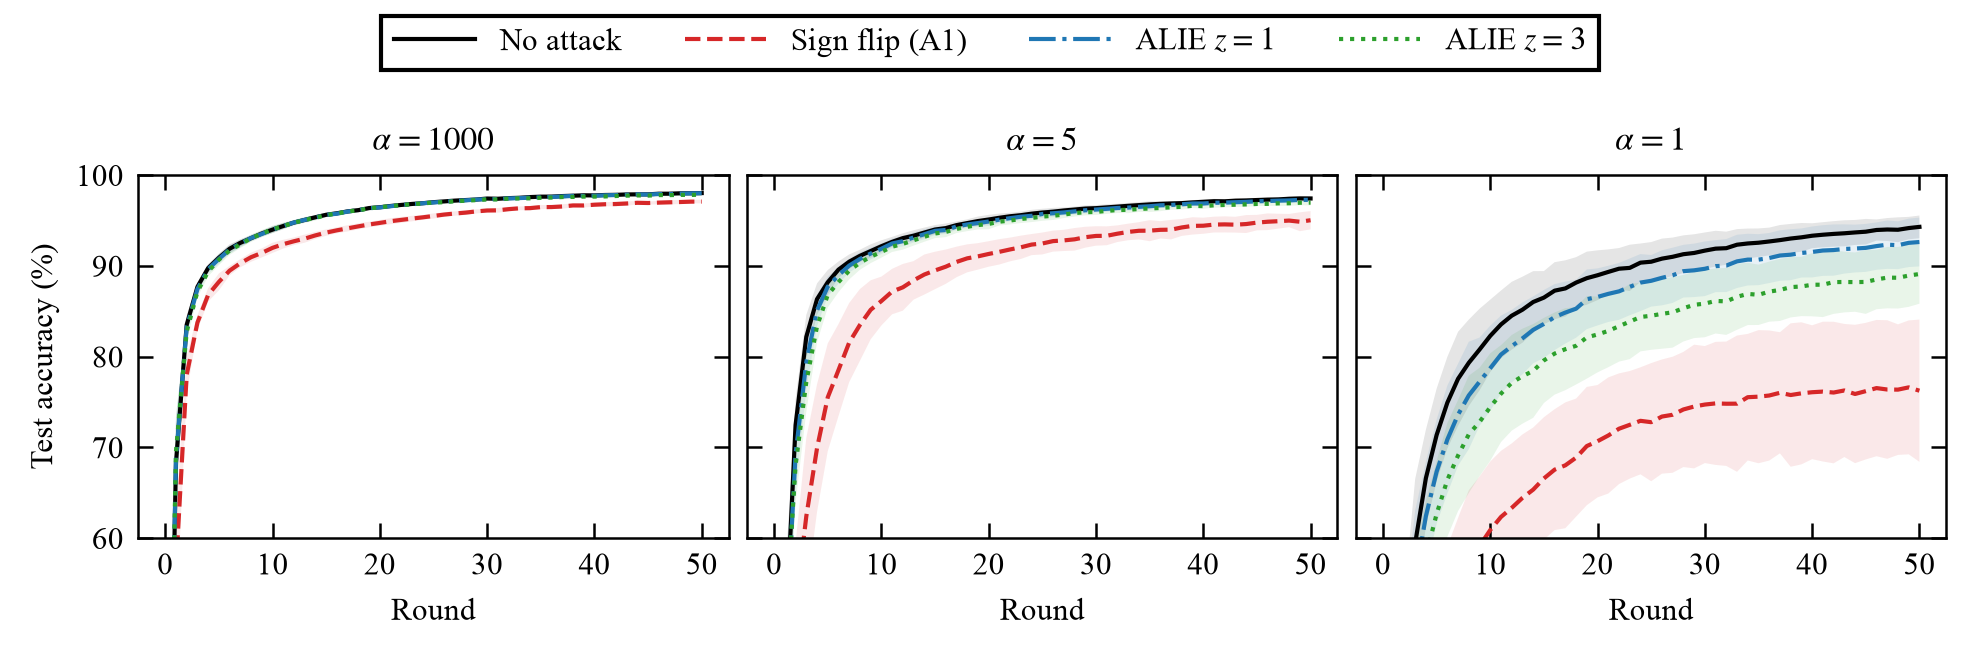
\includegraphics[width=0.75\textwidth]{fig/accuracy_by_round_v3.png}
\caption{テスト精度のラウンド推移（10試行の平均, 帯は$\pm$標準偏差）. ALIEは8水準の $z$ のうち $z=1$ と $z=3$ のみを示す. 縦軸は $60\%$ 以上を表示}
\label{fig:acc-round}
\end{figure*}

攻撃なしの条件の精度は $\alpha=1000,\,5,\,1$ でそれぞれ $98.0\%$, $97.4\%$, $94.3\%$ であった. 5ラウンドごとの精度の上がり幅を見ると, $\alpha=1000$ では第35ラウンド以降およそ $0.1$ ポイントで横ばいとなり, $\alpha=5$ でも第50ラウンドにかけて $0.2$ ポイント程度まで小さくなった. 一方, $\alpha=1$ では第45--50ラウンドでも $0.5$ ポイント程度と, $\alpha=1000$ の約4倍の速さでなお上昇していた. 攻撃ありの条件も同様の傾向であった（表\ref{tab:acc}）. したがって, $\alpha=1$ の第46--50ラウンドの検知性能は, 学習が進みきる前の段階のものである.

符号反転は, $\alpha=1000,\,5$ で精度をそれぞれ約 $0.9$, $2.4$ ポイント, $\alpha=1$ で約 $18$ ポイント低下させた. $\alpha=1$ の符号反転は試行間のばらつきも大きく（最低 $63.2\%$）, 精度は約 $76\%$ で頭打ちとなった. ALIEは, $\alpha=1000,\,5$ ではどの $z$ でも精度をほとんど変化させず, 攻撃なしとの差は最大 $0.5$ ポイントであった. $\alpha=1$ では $z$ とともに精度が低下し, $z \le 1.5$ では攻撃なしとの差が2ポイント以内であったのに対し, $z=2$ で約 $2.6$ ポイント, $z=3$ で約 $5.2$ ポイント低下した. すなわち, 本実験の設定（FedAvg）では, ALIEは $\alpha \ge 5$ では精度の観点で攻撃としてほとんど機能せず, Non-IIDが強く $z$ が大きい場合にのみ精度を下げた. 外れ値を除外しない単純な平均がこの攻撃に対して最もよい防御であったという原論文の報告\cite{baruch2019little}と整合する.

\subsection{検知性能の全体像}
\label{sec:res-final}

表\ref{tab:final-auc}に, 第46--50ラウンドのROC-AUCを, 図\ref{fig:auc-z}にALIEの $z$ とAUCの関係を示す.

\begin{table*}[t]
\centering
\caption{第46--50ラウンドのROC-AUC（試行ごとに第46--50ラウンドを平均したうえでの10試行の平均. 試行間の標準偏差が $0.10$ 以上のものは$\pm$で併記）}
\label{tab:final-auc}
\footnotesize
\tabcolsep=3.5pt
\begin{tabular}{@{}l@{\hspace{5pt}}cccc@{\hspace{8pt}}cccc@{\hspace{8pt}}cccc@{}}
\toprule
 & \multicolumn{4}{c}{$\alpha=1000$} & \multicolumn{4}{c}{$\alpha=5$} & \multicolumn{4}{c}{$\alpha=1$} \\
\cmidrule(lr){2-5}\cmidrule(lr){6-9}\cmidrule(l){10-13}
攻撃 & D1 & D2 & D3 & D4 & D1 & D2 & D3 & D4 & D1 & D2 & D3 & D4 \\
\midrule
A1 符号反転 & 0.97 & 1.00 & 1.00 & 1.00 & 0.94 & 1.00 & 0.99 & 0.97 & 0.88 & 1.00 & 0.98 & 0.85$\pm$0.12 \\
\midrule
A2 $z{=}0.385$ & 1.00 & 0.00 & 0.96 & 0.09 & 1.00 & 0.00 & 1.00 & 0.04 & 0.97 & 0.00 & 0.97 & 0.04 \\
A2 $z{=}0.5$ & 1.00 & 0.00 & 0.96 & 0.16$\pm$0.10 & 1.00 & 0.00 & 1.00 & 0.06 & 0.96 & 0.00 & 0.97 & 0.07 \\
A2 $z{=}0.75$ & 1.00 & 0.00 & 0.99 & 1.00 & 1.00 & 0.00 & 1.00 & 0.39$\pm$0.21 & 0.88$\pm$0.10 & 0.00 & 0.93$\pm$0.12 & 0.16$\pm$0.11 \\
A2 $z{=}1$ & 0.88 & 0.00 & 0.99 & 1.00 & 0.84 & 0.00 & 1.00 & 1.00 & 0.47$\pm$0.20 & 0.00 & 0.98 & 0.81$\pm$0.26 \\
A2 $z{=}1.25$ & 0.16 & 0.00 & 0.98 & 1.00 & 0.09 & 0.00 & 0.99 & 1.00 & 0.14$\pm$0.16 & 0.00 & 0.98 & 1.00 \\
A2 $z{=}1.5$ & 0.99 & 0.00 & 0.99 & 1.00 & 0.94 & 0.00 & 1.00 & 1.00 & 0.72$\pm$0.18 & 0.00 & 0.98 & 1.00 \\
A2 $z{=}2$ & 1.00 & 0.83$\pm$0.17 & 0.99 & 1.00 & 1.00 & 0.12$\pm$0.13 & 1.00 & 1.00 & 0.99 & 0.00 & 0.98 & 1.00 \\
A2 $z{=}3$ & 1.00 & 1.00 & 1.00 & 1.00 & 1.00 & 1.00 & 1.00 & 1.00 & 1.00 & 0.97 & 0.98 & 1.00 \\
\bottomrule
\end{tabular}
\end{table*}

\begin{figure*}[t]
\centering
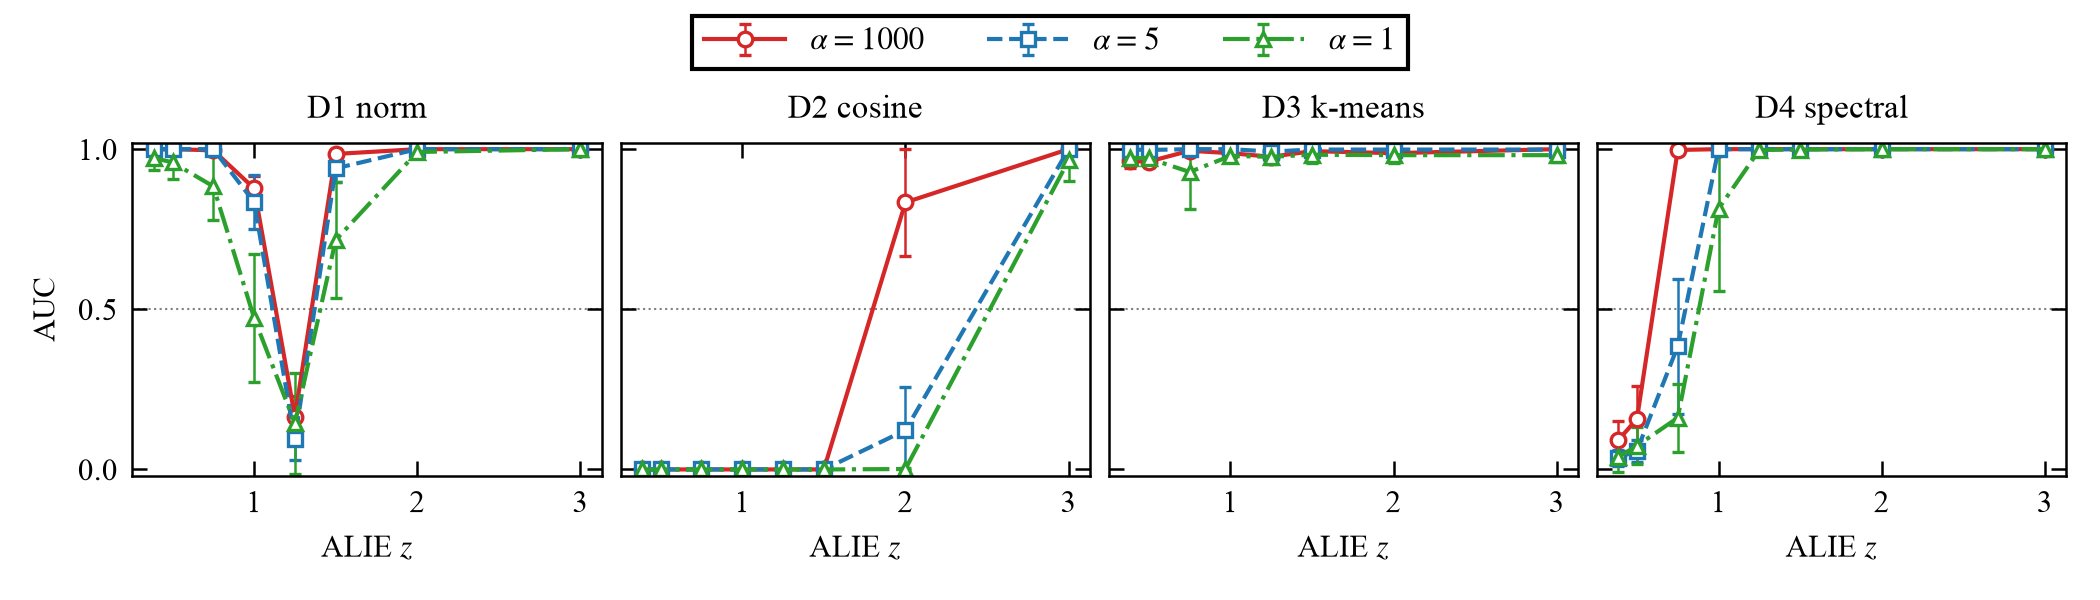
\includegraphics[width=\textwidth]{fig/detection_auc_by_z_v3.png}
\caption{ALIEの $z$ と第46--50ラウンドのAUC. 点は10試行の平均, 棒は$\pm$標準偏差. 赤実線○: $\alpha=1000$, 青破線□: $\alpha=5$, 緑一点鎖線△: $\alpha=1$. 点線は $\mathrm{AUC}=0.5$}
\label{fig:auc-z}
\end{figure*}

符号反転攻撃に対しては, D2・D3は全 $\alpha$ で $\mathrm{AUC} \ge 0.97$ を達成し, 想定どおり容易に検知できた. D1とD4は $\alpha$ が小さいほど低下し, $\alpha=1000,\,5,\,1$ の順にD1が $0.97$, $0.94$, $0.88$, D4が $1.00$, $0.97$, $0.85$ であった. D1は, ノルムを変えないはずの攻撃に対して $0.5$ を大きく上回った.

ALIEに対しては, D2は $z \le 1.5$ では全 $\alpha$ でAUCが $0.00$ であり, すべての悪性更新がすべての正常更新よりも「正常らしい」と評価され, 順位が完全に逆転した. $z=2$ ではAUCが $\alpha$ によって大きく異なり（$\alpha=1000,\,5,\,1$ の順に $0.83$, $0.12$, $0.00$）, $z=3$ では全 $\alpha$ で $0.96$ 以上となった.

D1のAUCは $z$ が小さいほど高く, $z \le 0.5$ では全 $\alpha$ で $0.95$ 以上であった. $z$ を大きくするとAUCは低下し, 全 $\alpha$ で $z=1.25$ において最小（$0.09$--$0.16$）となった. $z \ge 1.5$ では再び上昇し, $z \ge 2$ では全 $\alpha$ で $0.99$ 以上であった. $z=0.75$--$1.5$ では $\alpha=1$ が他の $\alpha$ より低く, 試行間のばらつきも大きかった.

D3は全条件で $\mathrm{AUC} \ge 0.92$ であり, $z$ にも $\alpha$ にもほとんど依存しなかった. D4は $z$ が小さいと $0.04$--$0.16$ と逆転し, ある $z$ を境に $1.0$ 近くへ切り替わった. $\alpha=1000,\,5$ では切り替わりは急であり, 切り替わる $z$ はそれぞれ $0.5$ と $0.75$ の間, $0.75$ と $1$ の間にあった. $\alpha=1$ では切り替わりがなだらかであり, AUCは $z=0.75$ で $0.16$, $z=1$ で $0.81$ であった. $z \ge 1.25$ では全 $\alpha$ で $1.00$ であった.

\subsection{AUCのラウンド推移}
\label{sec:res-rounds}

図\ref{fig:auc-round}に, 検知器ごとのAUCのラウンド推移（試行間の平均$\pm$標準偏差）を示す. 行が検知器, 列が攻撃に対応し, $\alpha$ は線の色・線種・マーカーで区別した. 図\ref{fig:auc-round}にはALIEの8水準のうち4水準のみを示し, 全8水準の推移は\ref{sec:appendix-rounds}の図\ref{fig:auc-round-all}に示す. 以下で述べる区間ごとの平均値（第1--5, 6--15, 16--30, 31--50ラウンド）は, 全条件について\ref{sec:appendix-segments}の表\ref{tab:seg-d1}--\ref{tab:seg-d4}に示す.

\begin{figure*}[t]
\centering
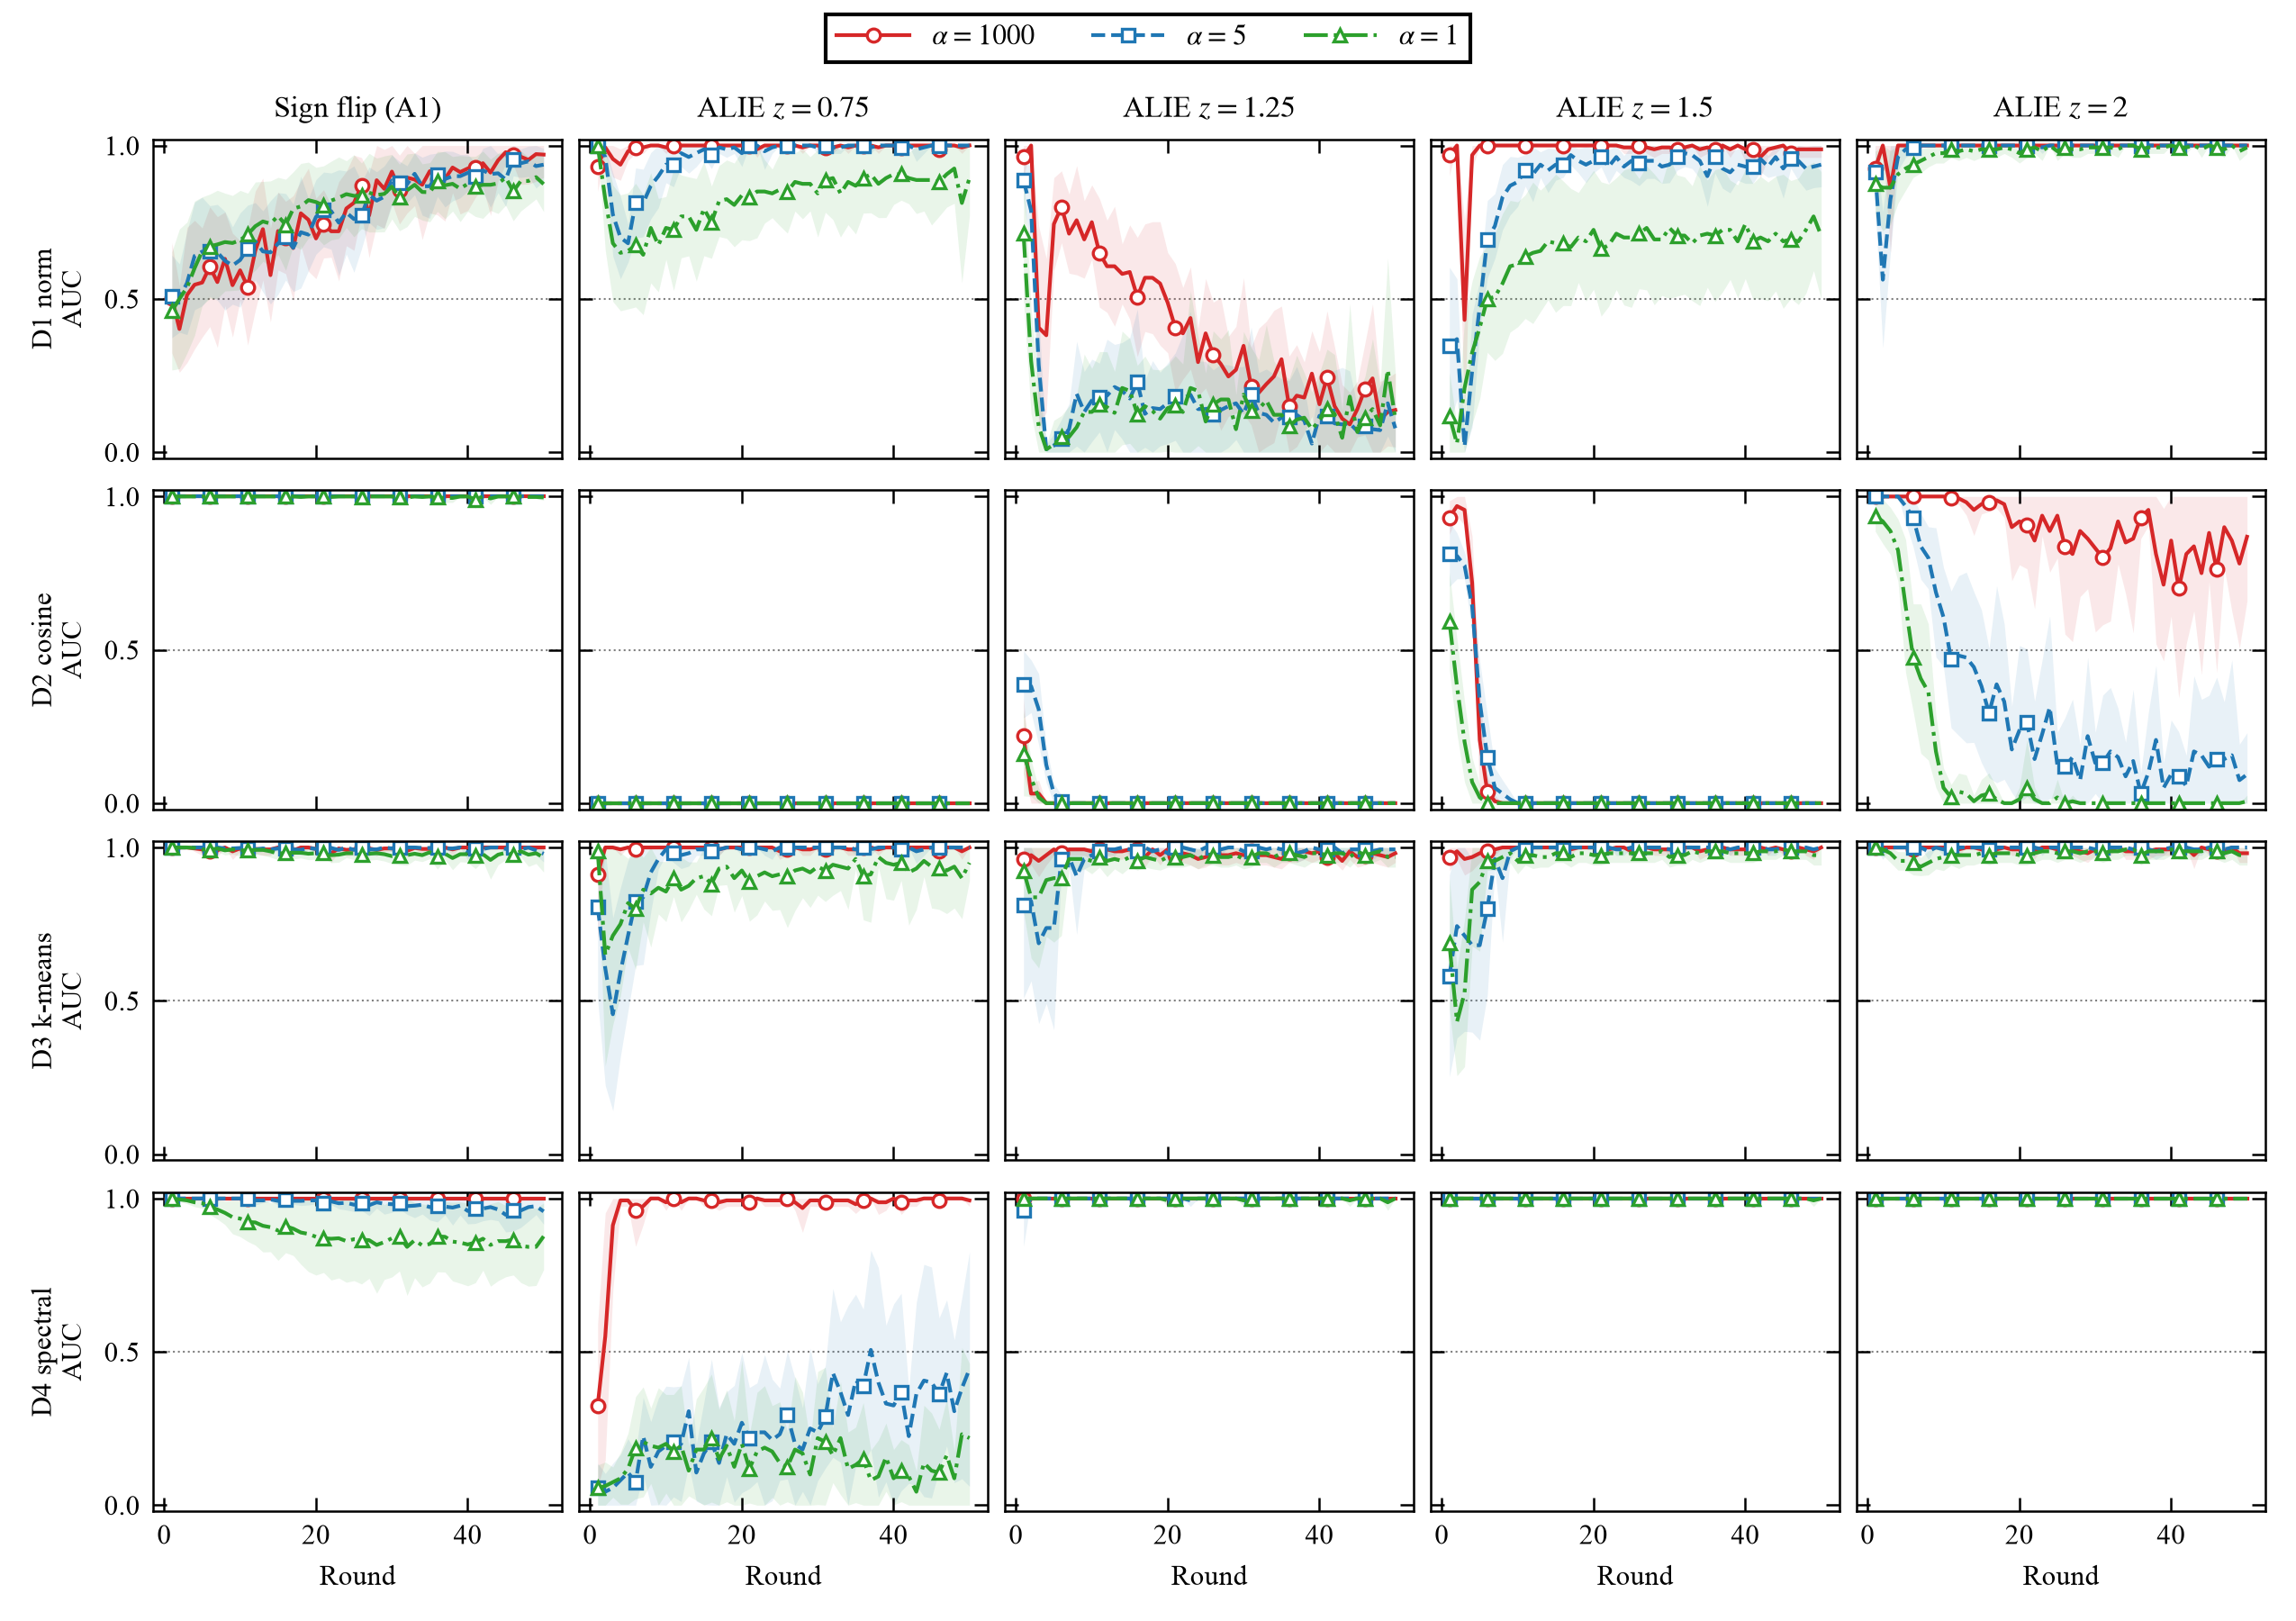
\includegraphics[width=\textwidth]{fig/detection_auc_by_round_v3_sel.png}
\caption{AUCのラウンド推移. 行は検知器D1--D4, 列は攻撃であり, ALIEは8水準のうち $z=0.75$, $1.25$, $1.5$, $2$ の4水準を示す（他の水準の第46--50ラウンドの値は表\ref{tab:final-auc}と図\ref{fig:auc-z}）. 線は試行間の平均, 帯は$\pm$標準偏差. 赤実線○: $\alpha=1000$, 青破線□: $\alpha=5$, 緑一点鎖線△: $\alpha=1$. 点線は $\mathrm{AUC}=0.5$}
\label{fig:auc-round}
\end{figure*}

ALIEでは, $z \le 1$ の全水準でD2のAUCが全ラウンドを通じて $0$ にとどまり（付録の図\ref{fig:auc-round-all}）, 順位の逆転は学習の初期から生じていた. 一方, $z=1.5$ のD2は第1--5ラウンドの平均が $0.25$--$0.76$ であったが, 第6--15ラウンドには $0.02$ 以下に下がった. $z=2$ のD2も, $\alpha=5,\,1$ では第1--5ラウンドの $0.99$, $0.84$ から第31--50ラウンドの $0.12$, $0.00$ へ低下した. D1は, $z=1.25$ の $\alpha=1000$ で第1--5ラウンドの $0.70$ から第31--50ラウンドの $0.18$ へ低下し, $z=1.5$ の $\alpha=1,\,5$ では $0.22$, $0.30$ から $0.71$, $0.94$ へ上昇した. D4は, $z=0.75$ の $\alpha=1000$ で第1--5ラウンドの $0.76$ から $0.99$ へ上昇し, $\alpha=5$ でも $0.07$ から $0.37$ へ緩やかに上昇した.

符号反転では, D2は全ラウンドで $1.00$, D3は $0.97$ 以上を維持した. D1は全 $\alpha$ で学習の進行とともに上昇した（第1--5ラウンドの $0.50$--$0.57$ から第31--50ラウンドの $0.87$--$0.93$）. D4は $\alpha=1$ でのみ, 第1--5ラウンドの $0.99$ から第31--50ラウンドの $0.86$ へ低下した.

このように, 検知性能は学習の段階によって大きく異なる場合がある. 特にD2がALIEを序盤には検知できていたこと（$z=1.5,\,2$）や, D4が符号反転を $\alpha=1$ でも序盤には検知できていたことは, 第46--50ラウンドの値（表\ref{tab:final-auc}）だけからは読み取れない.

\subsection{Non-IID度と正常更新のばらつき}
\label{sec:res-spread}

表\ref{tab:spread}に, 攻撃なし条件における \Spread{} と正常更新の第1主成分の寄与率を示す. Non-IIDが強いほど \Spread{} は大きかったが, その差は学習の段階に強く依存した. 第1--5ラウンドでは $\alpha=1000$ の $0.149$ に対して $\alpha=5,\,1$ は $0.353$, $0.434$ と約 $2.4$--$2.9$ 倍であったが, 第46--50ラウンドでは $1.00$--$1.08$ 倍にとどまった. 一方, 第1主成分の寄与率は第46--50ラウンドでも $\alpha=1000,\,5,\,1$ の順に $0.086$, $0.122$, $0.193$ と約 $2.2$ 倍の差があった.

\begin{table}[t]
\centering
\caption{攻撃なし条件における \Spread{} と正常更新の第1主成分の寄与率. 全ラウンドの値はラウンド単位の値の平均$\pm$標準偏差}
\label{tab:spread}
\small
\begin{tabular}{@{}lcccc@{}}
\toprule
 & \multicolumn{3}{c}{\Spread{}} & 寄与率 \\
\cmidrule(lr){2-4}\cmidrule(l){5-5}
$\alpha$ & 全ラウンド & 第1--5 & 第46--50 & 第46--50 \\
\midrule
1000 & $0.151 \pm 0.009$ & $0.149$ & $0.143$ & $0.086$ \\
5    & $0.182 \pm 0.070$ & $0.353$ & $0.143$ & $0.122$ \\
1    & $0.211 \pm 0.087$ & $0.434$ & $0.155$ & $0.193$ \\
\bottomrule
\end{tabular}
\end{table}

表\ref{tab:pushratio}に, 攻撃あり条件における第46--50ラウンド平均の \PushRatio{} を示す. ALIEの \PushRatio{} は $\alpha$ によらず $z$ の $1.00$--$1.02$ 倍であり, 式(\ref{eq:alie-pushratio})から予想されるとおり $z$ によってほぼ決まった. 符号反転の \PushRatio{} は, 第46--50ラウンドでは $\alpha=1000,\,5,\,1$ の順に $1.58$, $2.03$, $2.55$ と, Non-IIDが強いほど大きかった. 第1--5ラウンドでは逆に $8.62$, $2.85$, $1.96$ とNon-IIDが強いほど小さく, 学習の段階によって大小関係が入れ替わった（\ref{sec:appendix-pushratio}の表\ref{tab:seg-push}）. 第46--50ラウンドの符号反転の \PushRatio{} の平均は全 $\alpha$ で $1.5$ 以上であり, $1$ を下回ることはなかった.

\begin{table*}[t]
\centering
\caption{第46--50ラウンド平均の \PushRatio{}（10試行の平均）}
\label{tab:pushratio}
\begin{tabular}{@{}lccccccccc@{}}
\toprule
 & & \multicolumn{8}{c}{ALIE（$z$）} \\
\cmidrule(l){3-10}
$\alpha$ & 符号反転 & $0.385$ & $0.5$ & $0.75$ & $1$ & $1.25$ & $1.5$ & $2$ & $3$ \\
\midrule
1000 & 1.58 & 0.39 & 0.50 & 0.75 & 1.00 & 1.25 & 1.50 & 2.01 & 3.01 \\
5 & 2.03 & 0.39 & 0.50 & 0.75 & 1.00 & 1.25 & 1.51 & 2.01 & 3.01 \\
1 & 2.55 & 0.39 & 0.51 & 0.76 & 1.02 & 1.27 & 1.52 & 2.03 & 3.05 \\
\bottomrule
\end{tabular}
\end{table*}

\subsection{符号反転攻撃における \PushRatio{} とAUCの関係}
\label{sec:res-pushratio}

符号反転攻撃について, ラウンド単位の \PushRatio{} とAUCの散布図を図\ref{fig:pushratio}に示す. 表\ref{tab:corr}には, 両者のSpearman順位相関係数 $\rho$ を, 全体（各検知器 $1{,}500$ 点）と $\alpha$ ごと（各 $500$ 点）に分けて示す.

\begin{figure}[t]
\centering
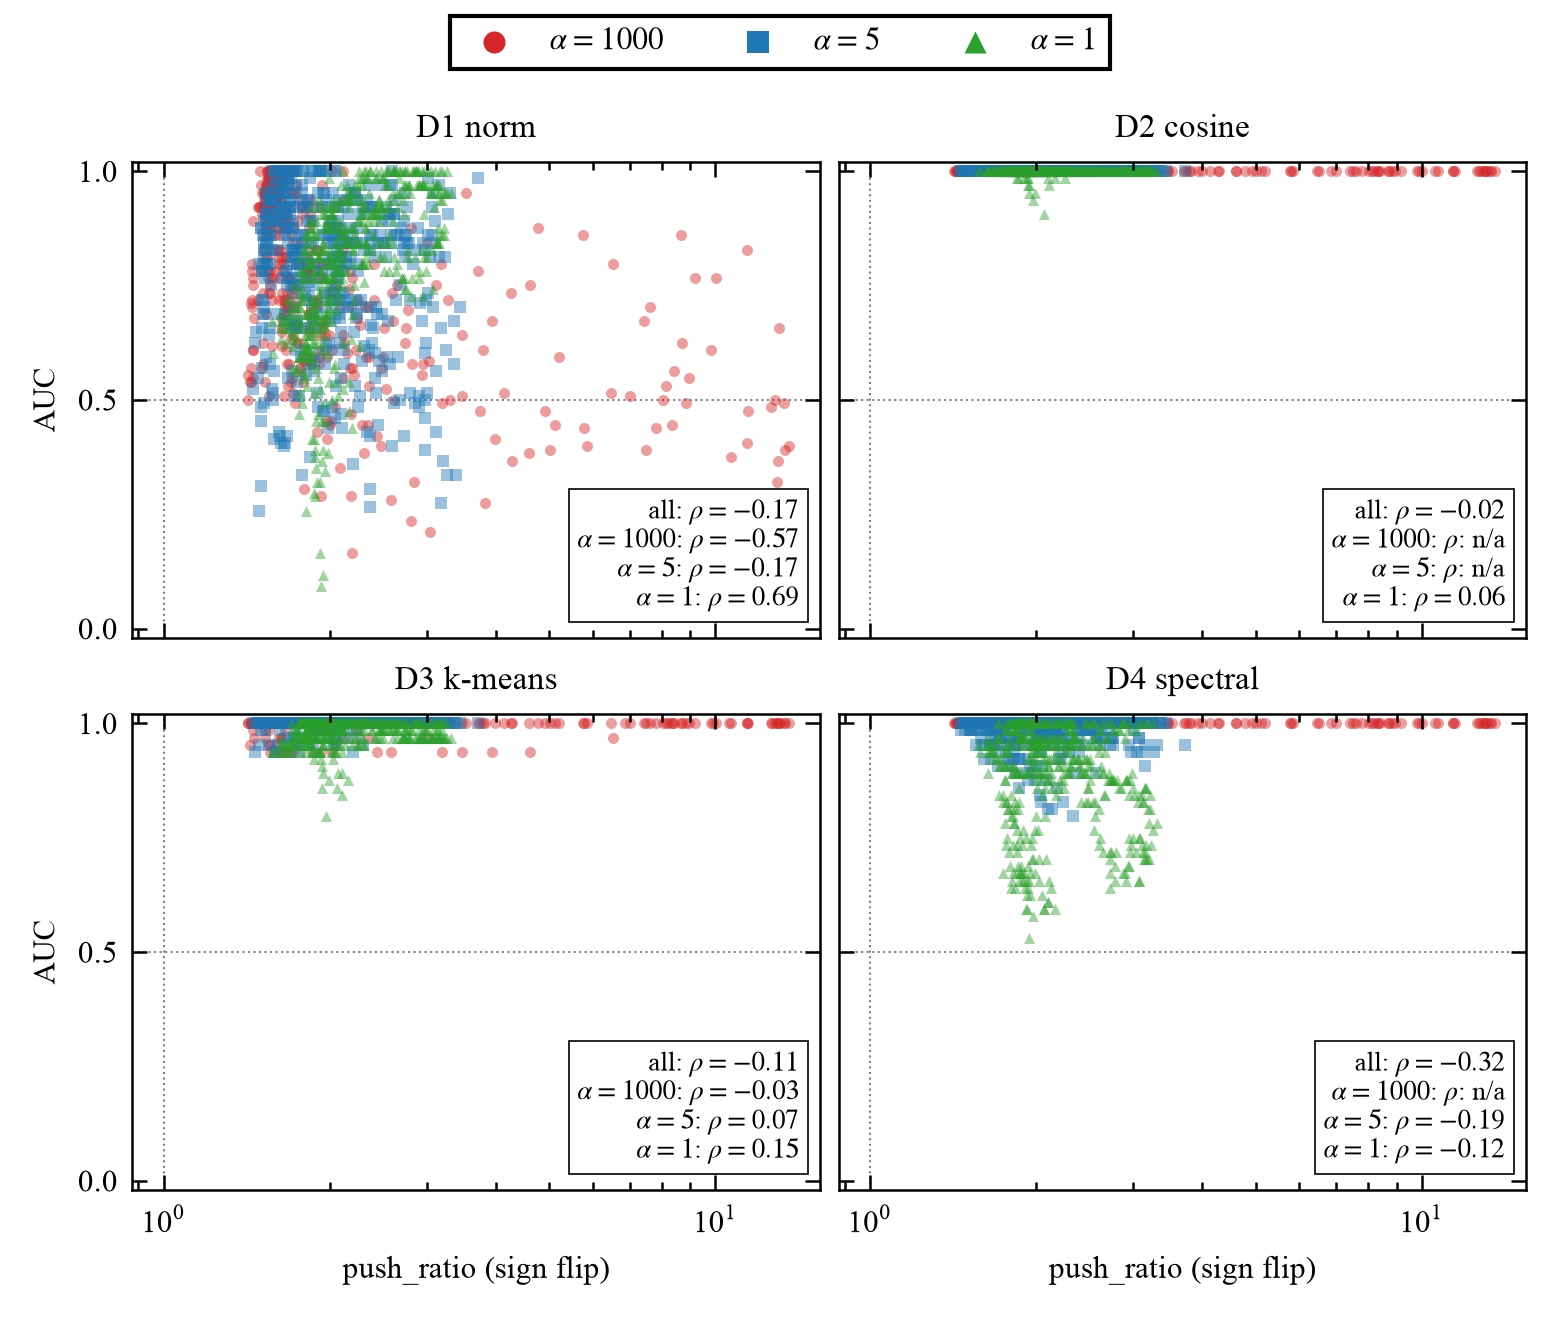
\includegraphics[width=\linewidth]{fig/detection_pushratio_vs_auc_v3.png}
\caption{符号反転攻撃における \PushRatio{}（横軸, 対数）とAUC（縦軸）の散布図. 1点が1実行の1ラウンドに対応する. 色と印は $\alpha$ を表す. 各パネル右下は順位相関係数（全体と $\alpha$ ごと. n/a はAUCが一定で計算できないもの）}
\label{fig:pushratio}
\end{figure}

\begin{table}[t]
\centering
\caption{符号反転攻撃における \PushRatio{} とAUCのSpearman順位相関係数 $\rho$（ラウンド単位, 同順位は平均順位で処理. n/a はAUCが一定で定義できないもの）}
\label{tab:corr}
\begin{tabular}{@{}lcccc@{}}
\toprule
 & 全体 & $\alpha=1000$ & $\alpha=5$ & $\alpha=1$ \\
\midrule
D1 & $-0.17$ & $-0.57$ & $-0.17$ & $\phantom{-}0.69$ \\
D2 & $-0.02$ & n/a & n/a & $\phantom{-}0.06$ \\
D3 & $-0.11$ & $-0.03$ & $\phantom{-}0.07$ & $\phantom{-}0.15$ \\
D4 & $-0.32$ & n/a & $-0.19$ & $-0.12$ \\
\bottomrule
\end{tabular}
\end{table}

\PushRatio{} とAUCの順位相関は, 全体でも $\alpha$ ごとでも弱いか負であった. 例外は $\alpha=1$ のD1（$\rho=0.69$）のみである. 図\ref{fig:pushratio}でも, \PushRatio{} が $1$ に近づくほどAUCが下がるという傾向は見られず, D2・D3は \PushRatio{} によらずほぼ $1$ であった.

\subsection{正常更新の分布構造}
\label{sec:res-structure}

表\ref{tab:structure}に, 第46--50ラウンドで平均した分布構造の指標（\ref{sec:metrics}節）を示す.

\begin{table*}[t]
\centering
\caption{第46--50ラウンド平均の分布構造の指標とD4のAUC（10試行の平均）. 寄与率は第1主成分の寄与率, $|\cos\theta|$ は悪性方向と第1主成分のなす角のコサインの絶対値であり, それぞれ正常更新のみ, および全更新（D4が用いるもの）について求めた. 順位は悪性値の座標ごとの順位の平均と標準偏差である}
\label{tab:structure}
\small
\begin{tabular}{@{}llccccccc@{}}
\toprule
 & & \multicolumn{2}{c}{寄与率} & \multicolumn{2}{c}{$|\cos\theta|$} & \multicolumn{2}{c}{順位} & \\
\cmidrule(lr){3-4}\cmidrule(lr){5-6}\cmidrule(lr){7-8}
$\alpha$ & 攻撃 & 正常 & 全更新 & 正常 & 全更新 & 平均 & 標準偏差 & D4のAUC \\
\midrule
1000 & A1 符号反転 & 0.102 & 0.183 & 0.051 & 0.994 & 0.563 & 0.261 & 1.000 \\
1000 & A2 $z{=}0.385$ & 0.102 & 0.099 & 0.051 & 0.079 & 0.339 & 0.143 & 0.091 \\
1000 & A2 $z{=}0.5$ & 0.102 & 0.097 & 0.049 & 0.118 & 0.298 & 0.143 & 0.158 \\
1000 & A2 $z{=}0.75$ & 0.102 & 0.110 & 0.048 & 0.920 & 0.224 & 0.143 & 0.998 \\
1000 & A2 $z{=}1$ & 0.101 & 0.171 & 0.044 & 0.993 & 0.167 & 0.149 & 1.000 \\
1000 & A2 $z{=}1.25$ & 0.101 & 0.241 & 0.044 & 0.998 & 0.124 & 0.157 & 1.000 \\
1000 & A2 $z{=}1.5$ & 0.101 & 0.313 & 0.044 & 0.999 & 0.094 & 0.167 & 1.000 \\
1000 & A2 $z{=}2$ & 0.101 & 0.446 & 0.047 & 1.000 & 0.064 & 0.190 & 1.000 \\
1000 & A2 $z{=}3$ & 0.100 & 0.644 & 0.051 & 1.000 & 0.073 & 0.248 & 1.000 \\
\midrule
5 & A1 符号反転 & 0.176 & 0.318 & 0.307 & 0.973 & 0.587 & 0.275 & 0.965 \\
5 & A2 $z{=}0.385$ & 0.142 & 0.138 & 0.039 & 0.051 & 0.342 & 0.143 & 0.036 \\
5 & A2 $z{=}0.5$ & 0.141 & 0.134 & 0.041 & 0.066 & 0.301 & 0.143 & 0.059 \\
5 & A2 $z{=}0.75$ & 0.141 & 0.128 & 0.040 & 0.305 & 0.225 & 0.146 & 0.385 \\
5 & A2 $z{=}1$ & 0.141 & 0.171 & 0.043 & 0.987 & 0.167 & 0.154 & 1.000 \\
5 & A2 $z{=}1.25$ & 0.140 & 0.241 & 0.045 & 0.998 & 0.124 & 0.166 & 1.000 \\
5 & A2 $z{=}1.5$ & 0.141 & 0.313 & 0.047 & 0.999 & 0.096 & 0.182 & 1.000 \\
5 & A2 $z{=}2$ & 0.141 & 0.447 & 0.050 & 1.000 & 0.075 & 0.216 & 1.000 \\
5 & A2 $z{=}3$ & 0.145 & 0.645 & 0.057 & 1.000 & 0.110 & 0.299 & 1.000 \\
\midrule
1 & A1 符号反転 & 0.298 & 0.410 & 0.403 & 0.958 & 0.612 & 0.269 & 0.854 \\
1 & A2 $z{=}0.385$ & 0.209 & 0.203 & 0.065 & 0.075 & 0.350 & 0.163 & 0.039 \\
1 & A2 $z{=}0.5$ & 0.206 & 0.197 & 0.060 & 0.078 & 0.307 & 0.166 & 0.074 \\
1 & A2 $z{=}0.75$ & 0.207 & 0.189 & 0.064 & 0.138 & 0.229 & 0.175 & 0.161 \\
1 & A2 $z{=}1$ & 0.208 & 0.191 & 0.073 & 0.704 & 0.170 & 0.189 & 0.814 \\
1 & A2 $z{=}1.25$ & 0.206 & 0.250 & 0.068 & 0.984 & 0.130 & 0.204 & 0.998 \\
1 & A2 $z{=}1.5$ & 0.206 & 0.320 & 0.064 & 0.993 & 0.108 & 0.223 & 0.999 \\
1 & A2 $z{=}2$ & 0.205 & 0.451 & 0.069 & 0.999 & 0.103 & 0.266 & 1.000 \\
1 & A2 $z{=}3$ & 0.215 & 0.648 & 0.081 & 1.000 & 0.180 & 0.371 & 1.000 \\
\bottomrule
\end{tabular}
\end{table*}

ALIEの悪性方向 $\bar{g}_M - \bar{g}_B$ は, 正常更新のみの第1主成分とはほぼ直交していた（$|\cos\theta| \le 0.08$）. 一方, 全更新の第1主成分との $|\cos\theta|$ は $z$ と $\alpha$ によって大きく異なり, D4のAUCとよく対応した（ALIEの24条件で $\rho=0.92$, ラウンド単位で $\rho=0.85$）. 例えば $z=0.75$ では, 全更新の第1主成分との $|\cos\theta|$ が $\alpha=1000,\,5,\,1$ の順に $0.920$, $0.305$, $0.138$ であり, D4のAUC（$0.998$, $0.385$, $0.161$）と対応した.

悪性値の座標ごとの順位の平均は, $z \le 1$ では全 $\alpha$ で正規分布から予想される $\Phi(-z)$（$z=0.385,\,0.5,\,0.75,\,1$ に対して $0.350$, $0.309$, $0.227$, $0.159$）とよく一致した（\ref{sec:appendix-rank}の表\ref{tab:rank}）. しかし $z \ge 1.25$ では $\Phi(-z)$ より大きく（例えば $z=3$ では $\Phi(-3) \approx 0.001$ に対して $0.073$--$0.180$）, その差はNon-IIDが強いほど大きかった. 標準偏差も $z$ とともに増加した（$0.14$--$0.37$）. すなわち, 正常更新の各座標の分布は, 中心付近では正規分布でよく近似できるが, 裾は正規分布より重く, Non-IIDが強いほどその傾向が強い.

% =========================================================
\section{考察}
\label{sec:discussion}

\subsection{検知器間の違い}
\label{sec:disc-detectors}

符号反転攻撃に対しては, D2とD3が全 $\alpha$ で高い検知性能を示した（表\ref{tab:final-auc}）. また, 図\ref{fig:auc-round}に示すように, D2とD3は学習の序盤から高いAUCを示した.

\begin{figure}[t]
\centering
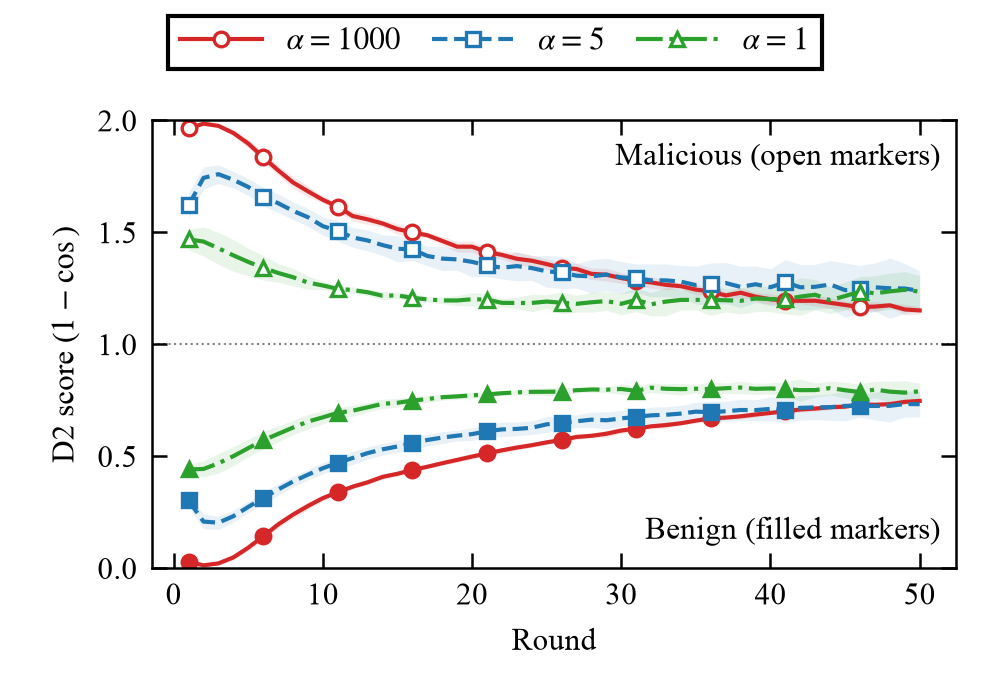
\includegraphics[width=\linewidth]{fig/signflip_d2_score_by_round_v3.png}
\caption{符号反転攻撃におけるD2スコア（参照方向へのコサイン距離）のラウンド推移. 白抜きの印は悪性更新, 塗りつぶしの印は正常更新の平均を表す（10試行の平均, 帯は$\pm$標準偏差）. 赤実線○: $\alpha=1000$, 青破線□: $\alpha=5$, 緑一点鎖線△: $\alpha=1$. 点線は $\cos\theta=0$ に対応するスコア $1$}
\label{fig:signflip-d2}
\end{figure}

\begin{table}[t]
\centering
\caption{符号反転攻撃における正常更新と悪性更新の分離（10試行の平均）. D2スコアは参照方向へのコサイン距離, 完全分離はラウンド内ですべての悪性更新のD2スコアがすべての正常更新を上回ったラウンドの割合, $|\cos|$ は悪性方向と全更新の第1主成分のなす角のコサインの絶対値}
\label{tab:signflip-sep}
\small
\tabcolsep=3pt
\begin{tabular}{@{}c@{\hspace{4pt}}cccc@{}}
\toprule
 & \multicolumn{2}{c}{D2スコア} & & \\
$\alpha$ & 正常 & 悪性 & 完全分離 & $|\cos|$ \\
\midrule
\multicolumn{5}{@{}l}{第1--5ラウンド} \\
1000 & $0.04$ & $1.95$ & $1.00$ & $1.00$ \\
5    & $0.24$ & $1.71$ & $1.00$ & $1.00$ \\
1    & $0.48$ & $1.43$ & $1.00$ & $0.99$ \\
\midrule
\multicolumn{5}{@{}l}{第46--50ラウンド} \\
1000 & $0.74$ & $1.16$ & $1.00$ & $0.99$ \\
5    & $0.73$ & $1.25$ & $1.00$ & $0.97$ \\
1    & $0.79$ & $1.24$ & $0.94$ & $0.96$ \\
\bottomrule
\end{tabular}
\end{table}

D2が符号反転を検知できるのは, 正常更新が共通の方向を持つためと考えられる. 正常更新 $g$ と参照方向 $r$ のなす角を $\theta$ とすると, 符号を反転した悪性更新 $-g$ と $r$ のなす角は $\pi-\theta$ となる. このとき, D2スコアは正常更新で $1-\cos\theta$, 悪性更新で $1+\cos\theta$ となる. したがって, 正常更新が参照方向と同じ側（$\cos\theta>0$）にある限り, 正常更新のスコアは $1$ 未満, 悪性更新のスコアは $1$ より大きくなり, 両者の順位は必ず分かれる. これは攻撃そのものの幾何的な性質によるものであり, 学習の段階によらない. 実際, 図\ref{fig:signflip-d2}に示すように, 学習の序盤には正常更新と悪性更新のスコアが $1$ を挟んでほぼ対称に分かれており, 第1--5ラウンドのスコアの平均は, $\alpha=1000$ で正常更新が $0.04$, 悪性更新が $1.95$ であった（表\ref{tab:signflip-sep}）.

一方, この性質は正常更新が共通の方向を持つことを前提としている. 正常更新の向きがばらつき, $\cos\theta$ が $0$ に近づくと, 正常更新と悪性更新のスコアの差 $2\cos\theta$ は小さくなる. 実際, 図\ref{fig:signflip-d2}では学習が進むにつれて両者のスコアが $1$ に近づき, 第46--50ラウンドの平均は, $\alpha=1000$ で正常更新が $0.74$, 悪性更新が $1.16$ と差が縮んでいた. また, $\alpha$ が小さいほど, 序盤から両者のスコアは $1$ に近かった. $\alpha=1$ の第46--50ラウンドでは, スコアが $1$ を超える正常更新が現れ, ラウンド内で悪性更新と正常更新が完全に分かれた割合は $0.94$ であった. したがって, 学習が進んだ場合やNon-IIDがさらに強い場合には, 正常更新の向きが揃わなくなり, D2による検知が難しくなる可能性がある. また, 参照方向 $r$ は全更新の座標ごとの中央値であるため, この議論は悪性クライアントが少数派であることも前提としている.

D3は, 更新のノルム, D2スコア, および第1・第2主成分への射影を特徴量とする（\ref{sec:detectors}節）. 符号反転では, 正常更新が共通の方向を向き, 悪性更新がその逆を向くため, 全更新を中心化した後の第1主成分は両者を結ぶ軸となる. 実際, 悪性方向と全更新の第1主成分の $|\cos|$ は, 全 $\alpha$ で第1--5ラウンドに $0.99$ 以上, 第46--50ラウンドに $0.96$ 以上であった（表\ref{tab:signflip-sep}）. そのため, 悪性更新はD2スコアでも第1主成分への射影でも正常更新と反対側に位置し, 2クラスタリングによって分離されやすい. すなわち, D3の高い検知性能は, 正常更新が共通の方向を持つという, D2と同じ性質によって支えられていると考えられる. なお, 符号反転は更新の大きさを変えないため, 学習の序盤ではノルムは分離に寄与しにくい. ただし学習が進むと悪性更新のノルムが大きくなるため（後述）, 終盤ではノルムも寄与している可能性がある.

\begin{figure}[t]
\centering
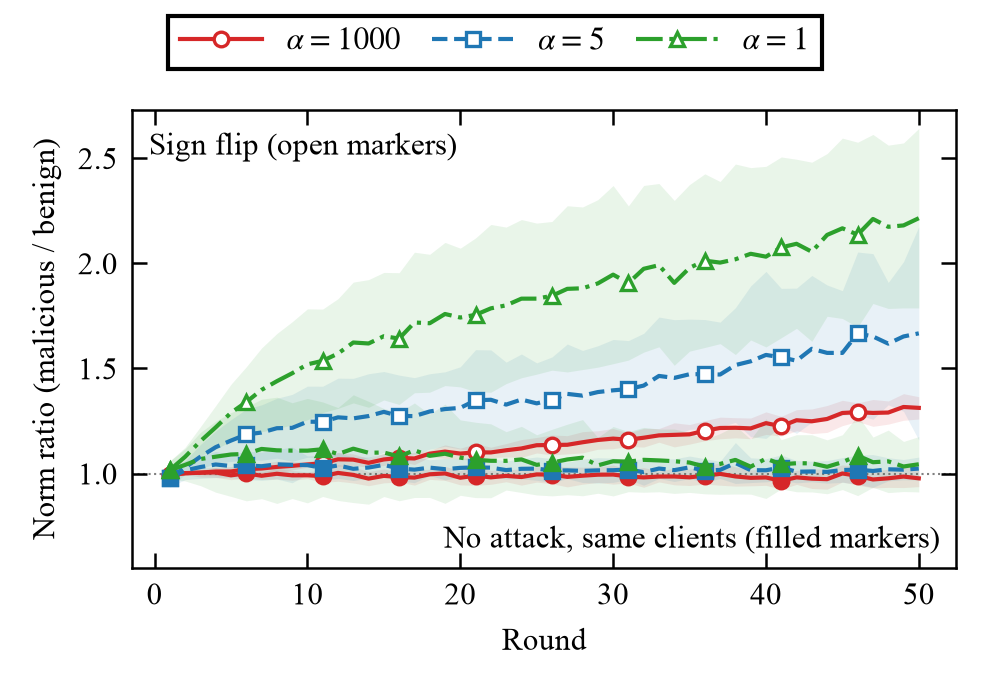
\includegraphics[width=\linewidth]{fig/signflip_norm_ratio_by_round_v3.png}
\caption{悪性更新のノルムの正常更新に対する比のラウンド推移. 白抜きの印は符号反転攻撃, 塗りつぶしの印は攻撃なしの条件で, 同じ試行で符号反転のときに悪性となる4台を悪性とみなした場合を表す（10試行の平均, 帯は$\pm$標準偏差）. 赤実線○: $\alpha=1000$, 青破線□: $\alpha=5$, 緑一点鎖線△: $\alpha=1$. 点線は比 $1$}
\label{fig:signflip-norm}
\end{figure}

\begin{table}[t]
\centering
\caption{符号反転攻撃の第46--50ラウンドにおけるノルムのばらつきとD1・D4の誤り（10試行の平均）. 比は悪性更新のノルムの正常更新に対する比, 変動係数は正常更新のノルムの標準偏差を平均で割ったもの, 誤りは検知器が悪性更新より正常更新を疑わしいと判定した組（正常1台と悪性1台）の割合, 下側（上側）は誤った組のうち正常更新のノルムが中央値より小さい（大きい）ものの割合, 相関は正常更新どうしでのD4のスコアとノルムの順位相関. -- は誤った組がないもの}
\label{tab:signflip-norm}
\footnotesize
\tabcolsep=2.2pt
\begin{tabular}{@{}c@{\hspace{3pt}}ccc@{\hspace{5pt}}cc@{\hspace{5pt}}ccc@{}}
\toprule
 & & \multicolumn{2}{c}{変動係数} & \multicolumn{2}{c}{D1} & \multicolumn{3}{c}{D4} \\
\cmidrule(lr){3-4}\cmidrule(lr){5-6}\cmidrule(l){7-9}
$\alpha$ & 比 & 符号反転 & 攻撃なし & 誤り & 下側 & 誤り & 上側 & 相関 \\
\midrule
1000 & $1.30$ & $0.08$ & $0.09$ & $0.035$ & $0.73$ & $0.000$ & -- & $0.51$ \\
5    & $1.65$ & $0.17$ & $0.09$ & $0.057$ & $0.60$ & $0.035$ & $0.82$ & $0.74$ \\
1    & $2.18$ & $0.39$ & $0.19$ & $0.122$ & $0.55$ & $0.146$ & $0.70$ & $0.78$ \\
\bottomrule
\end{tabular}
\end{table}

D1は各クライアントの更新の大きさと全クライアントの中央値との差をスコアとするため, 符号反転攻撃の本質である向きの反転を検知する仕組みを持たない. そのため, 向きが逆でも正常更新と同じ大きさの悪性更新は区別できず, 図\ref{fig:auc-round}に示すように, 学習の序盤のAUCは $0.5$ 付近, すなわちランダムな判定に近い値であったと考えられる.

一方, D1のAUCはラウンドが進むにつれて上昇した. 図\ref{fig:signflip-norm}に示すように, 攻撃なしの条件では, 同じ4台のクライアントのノルムの正常更新に対する比は全ラウンドを通じてほぼ $1$ にとどまったことから, この上昇は攻撃によって生じたものである. 符号反転は更新の大きさを変えないため, 悪性更新のノルムは, 悪性クライアントがローカル学習で計算した更新のノルムに等しい. 集約時には悪性クライアントの更新が反転して加えられるため, グローバルモデルは悪性クライアントのデータに適合する方向とは逆向きに動かされる. その結果, グローバルモデルは悪性クライアントのデータに適合しにくくなり, 悪性クライアントのローカル学習では損失が大きく, 更新も大きくなると考えられる. これが積み重なることでノルムの差が開き, AUCが上昇したと推測できる. 実際, 悪性更新のノルムの正常更新に対する比は, 第1--5ラウンドの $1.00$--$1.15$ から第46--50ラウンドの $1.30$--$2.18$ へと増大した. ただし, クライアントごとのローカル学習の損失は記録していないため, この機構は直接には確かめていない.

また, ノルムの比が最も大きい $\alpha=1$ において, D1のAUCは最も低かった. これは, Non-IIDが強いほど正常更新どうしのノルムのばらつきが大きいためと考えられる. 表\ref{tab:signflip-norm}に示すように, 第46--50ラウンドにおける正常更新のノルムの変動係数は, $\alpha=1000,\,5,\,1$ の順に $0.08$, $0.17$, $0.39$ であった. D1は中央値からの差の絶対値をスコアとするため, ノルムが中央値から大きく離れた正常更新は, 大きい側であっても小さい側であっても悪性更新と同程度に疑わしいと判定される. 実際, D1が悪性更新よりも正常更新を疑わしいと判定した組のうち, $\alpha=1$ では $55\%$ が中央値より小さいノルムの正常更新によるものであった. Non-IIDでラベルの偏りが強いと, クライアントごとにグローバルモデルへの適合の度合いが異なるため, 正常更新のノルムもばらつくと考えられる. 攻撃なしの条件でも, 正常更新のノルムの変動係数は $\alpha=1$ で $0.19$ と, $\alpha=1000$ の $0.09$ の約2倍であった. さらに, $\alpha=1$ では符号反転のもとでの変動係数（$0.39$）が攻撃なし（$0.19$）の約2倍であり, 攻撃そのものも正常更新のノルムのばらつきを広げていた.

符号反転に対するD4のAUCは, $\alpha=1$ では学習の序盤には $0.99$ であったが, 第46--50ラウンドには $0.85$ まで低下した. 一方, 悪性方向と全更新の第1主成分の $|\cos|$ はこの区間でも $0.96$ であり（表\ref{tab:signflip-sep}）, AUCが最も低かったラウンド（$0.59$）でも $0.92$ であった. すなわち, 第1主成分は悪性方向を捉えているにもかかわらず, 検知性能が低下していた.

これは, D4のスコアが第1主成分への射影の2乗であり, 射影の符号が失われるためと考えられる. 符号反転では, 第1主成分は正常更新が共通に向く方向とほぼ一致するため, 中心化した後の射影は, 正常更新が一方の側, 悪性更新がその反対側に位置すると考えられる. 射影を2乗すると, 負の側にある悪性更新のスコアも正となり, 中心から遠い正常更新と区別できなくなる. ノルムの大きい正常更新は, 共通の方向に沿って中心から遠くに位置するため, 悪性更新と同程度のスコアを持ちうる. 実際, 表\ref{tab:signflip-norm}に示すように, $\alpha=1$ の第46--50ラウンドでは, 正常更新のD4のスコアとノルムの順位相関は $0.78$ であり, D4が悪性更新より正常更新を疑わしいと判定した組のうち $70\%$ は, ノルムが中央値より大きい正常更新によるものであった. $\alpha=1$ では正常更新のノルムのばらつきが大きいため, このような正常更新が多く, AUCが低下したと考えられる. なお, 射影の値そのものは記録していないため, 正常更新と悪性更新が第1主成分上で反対側に位置することは, $|\cos|$ とスコアの関係から推測したものである.

D1とD4は, D2・D3に比べて学習の段階やNon-IID度によるAUCの変動が大きかった（D1では序盤にランダムに近く, その後上昇した. D4ではNon-IIDが強い条件で学習の進行とともに低下した）. D1は更新の大きさのみを用い, D4は第1主成分への射影の2乗を用いるため, いずれも正常更新の共通の方向に対して悪性更新が反対側にあるという, 符号反転の最も直接的な特徴（符号）を用いていない. そのため, これらの検知器の判定は中心からの離れ具合に依存し, 正常更新のノルムのばらつきに左右される. 実際, $\alpha=1$ では, 正常更新のノルムの変動係数が第1--5ラウンドの $0.18$ から第31--50ラウンドの $0.37$ へと広がり, それとともにD4のAUCは $0.99$ から $0.86$ へ低下した. 攻撃なしの条件では変動係数は $0.18$--$0.25$ にとどまっており, このばらつきの拡大は攻撃によって生じたものと考えられる. これに対し, D2は参照方向とのなす角のコサインの符号によって正常更新と悪性更新を分けることができ, D3はD2スコアを特徴量に含むため, 学習の段階やNon-IID度によらず高い検知性能を保ったと考えられる.

ALIEに対しては, D2のAUCは $z \le 1.5$ のすべての条件で $0.00$ であった（表\ref{tab:final-auc}）. これは悪性と正常を区別できないことを意味するのではなく, すべての悪性更新がすべての正常更新よりも正常らしいと判定され, 順位が完全に逆転していることを意味する.

ALIEの悪性更新は正常更新の平均の近くに置かれ（式(\ref{eq:alie})）, $z<1$ では平均からの距離は正常更新より悪性更新のほうが小さくなる. D2の参照方向 $r$ は全更新の座標ごとの中央値であり, 4台の悪性更新はすべて同じベクトルで, どの座標でも平均より下の同じ側に位置するため, $r$ は悪性更新の側へ寄る. 一方, 正常更新のずれは座標ごとに向きがばらばらであり, 中央値では打ち消し合う. 学習が進んだ段階では正常更新の平均そのものは小さいため, $r$ の向きは主に悪性方向へのずれによって決まる. そのため, 平均からの距離が正常更新とほぼ等しい $z=1$ でも, 第46--50ラウンドにおける悪性更新のD2スコアの平均は $0.22$--$0.33$ と, 正常更新の $0.89$--$1.01$ より小さかった.

また, 正常更新のD2スコアがほぼ $1$ であることは, $\cos\theta \approx 0$, すなわち正常更新が $r$ とほぼ直交することを意味する. 正常更新を平均 $\mu$ と各クライアントのずれ $e_i$ の和 $\mu + e_i$ と表すと, $\mu$ は小さいため, 正常更新と $r$ の角度はほぼ $e_i$ と悪性方向 $-z\sigma$ の角度で決まる. 両者のなす角のコサインは, 更新ベクトルの次元数を $d$ として
\begin{equation}
\cos\theta = \frac{\sum_{j=1}^{d} e_{ij}\,(-z\sigma_j)}{\|e_i\|\,\|z\sigma\|}
\end{equation}
であり, 分子の内積は, 座標 $j$ を標本とみなした共分散 $\operatorname{Cov}_j$ と座標の平均 $\bar{e}_i,\ \bar{\sigma}$ を用いて
\begin{equation}
\sum_{j=1}^{d} e_{ij}\,\sigma_j = d\left(\operatorname{Cov}_j(e_{ij}, \sigma_j) + \bar{e}_i\,\bar{\sigma}\right)
\end{equation}
と分解できる. $e_i$ は平均からのずれであるため $\bar{e}_i \approx 0$ であり, 内積がほぼ $0$ であることは, 座標ごとに見て $e_{ij}$ と $\sigma_j$ に相関がないことに対応する. $\sigma_j$ は各座標の標準偏差であり, すべての座標で正であるのに対し, $e_{ij}$ の符号は座標ごとにばらばらであるため, 両者に相関はほとんどなく, 高次元では $e_i$ と悪性方向はほぼ直交する. このため, 悪性更新が正常更新よりも正常らしいと判定され, $z \le 1.5$ ではAUCが $0.00$ になったと考えられる. なお, $r$ や $e_i$ そのものは記録していないため, この説明はD2スコアの値から推測したものである.

\begin{figure}[t]
\centering
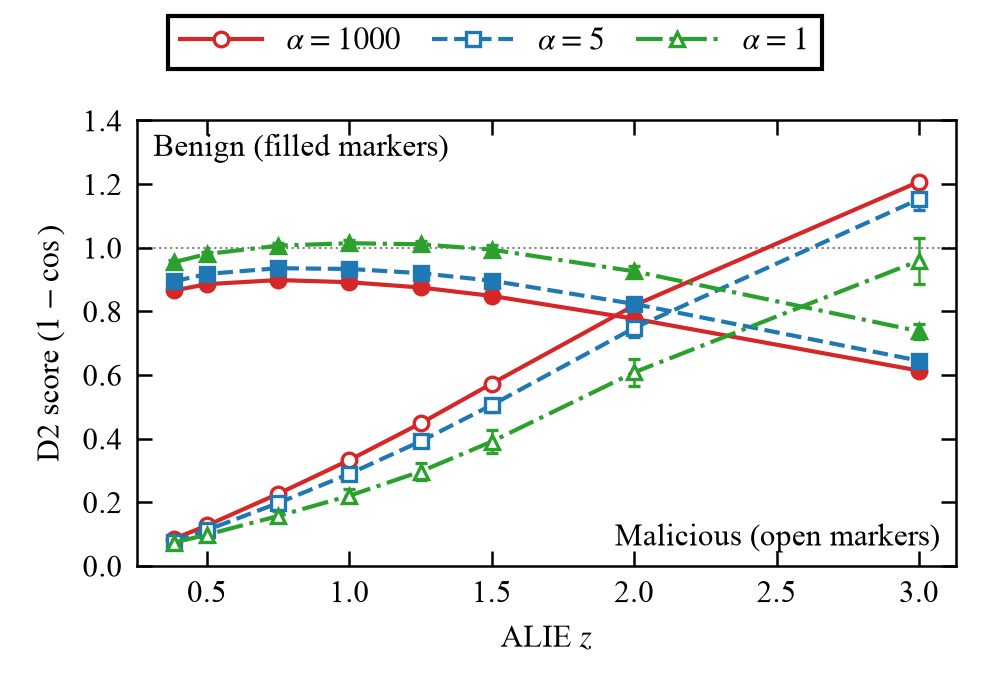
\includegraphics[width=\linewidth]{fig/alie_d2_score_by_z_v3.png}
\caption{ALIEの $z$ と第46--50ラウンドのD2スコア（参照方向へのコサイン距離）. 塗りつぶしの印は正常更新, 白抜きの印は悪性更新の平均を表す（10試行の平均, 棒は$\pm$標準偏差）. 赤実線○: $\alpha=1000$, 青破線□: $\alpha=5$, 緑一点鎖線△: $\alpha=1$. 点線は $\cos\theta=0$ に対応するスコア $1$}
\label{fig:alie-d2-z}
\end{figure}

D2が検知に転じる $z$ は $\alpha$ によって異なり, $\alpha=1000$ では $z=2$ でAUCが $0.83$ となったのに対し, $\alpha=1$ では $z=2$ でも $0.00$ であり, $z=3$ でようやく $0.97$ となった. 図\ref{fig:alie-d2-z}に示すように, $z$ を大きくすると悪性更新は平均から離れ, $r$ とのなす角が大きくなる. 悪性更新のスコアが正常更新のスコアを上回った $z$ で, D2は検知に転じる. Non-IIDが強いと, 各クライアントの更新は自身のラベルに合う方向へクライアントごとに異なる向きを向くため, 平均すると互いに打ち消し合い, 共通の成分 $\mu$ は各クライアントのずれ $e_i$ に比べて小さくなる. 実際, 攻撃なしの条件における第46--50ラウンドの正常更新のD2スコアは, $\alpha=1000,\,5,\,1$ の順に $0.81$, $0.84$, $0.90$ であった. $\mu$ が相対的に小さいほど, 正常更新は $r$ と直交に近くなり, 一方で $r$ の向きは悪性方向へのずれによってより強く決まる. そのため, $\alpha=1$ では正常更新のスコアが大きく（$z=1$ で $1.01$）, 悪性更新のスコアが小さく（$z=1$ で $0.22$）, 両者が交わる $z$ が大きくなったと考えられる.

D3は, ALIEに対してもすべての条件でAUC $0.92$ 以上を示した. D3のスコアは, 標準化した特徴量の空間における正常クラスタの重心からの距離であり, 重心からどちらの向きに外れても大きくなる. ALIEの悪性更新のD2スコアは正常更新を大きく下回っており（図\ref{fig:alie-d2-z}）, D2では「スコアが大きいほど悪性」という片側の規則のために順位が逆転したが, D3ではこの外れ方も重心から離れていることとして検出される. 加えて, ALIEでは悪性クライアント4台が同一のベクトルを送るため, 悪性更新は特徴量の空間で1点に重なり, 2クラスタリングによって分離されやすい. ただし, この性質は原論文の更新生成則に由来するものであり, 悪性更新に小さなばらつきを持たせた場合にも同じ結果が得られるかは確認していない.

D1のAUCは, ALIEの $z$ に対してU字型の変化を示し, $z \le 0.5$ では全 $\alpha$ で $0.95$ 以上, $z=1.25$ で最小（$0.09$--$0.16$）となり, $z \ge 2$ では再び $0.99$ 以上となった（表\ref{tab:final-auc}）. 第46--50ラウンドにおける悪性更新のノルムの正常更新に対する比は, $z=0.385$ で $0.37$--$0.40$, $z=1$ で $0.84$--$0.85$, $z=1.25$ で $1.03$--$1.04$, $z=1.5$ で $1.21$--$1.23$ であった. D1は中央値からの差の絶対値をスコアとするため, 悪性更新のノルムが小さすぎても大きすぎても検知でき, 両者のノルムが揃う $z=1.25$ 付近で見分けられなくなる. このとき悪性更新4台は同じノルムを持ち中央値の近くに位置するため, 正常更新よりも正常らしいと判定され, AUCは $0.5$ を下回った. 符号反転の $\alpha=1$ と同様に, D1は悪性更新のノルムが正常更新のノルムの分布と重なると検知できない. なお, $z$ が小さいときに悪性更新のノルムが正常更新より小さくなる理由は\ref{sec:disc-rq3}節で論じる.

D4のAUCは, $z$ が小さいと $0.04$--$0.16$ と逆転し, ある $z$ を境に $1.0$ 近くへ切り替わった. 切り替わる $z$ は, $\alpha=1000$ では $0.5$ と $0.75$ の間, $\alpha=5,\,1$ では $0.75$ と $1$ の間にあった. ただし, $\alpha=1$ では切り替わりがなだらかであり, $z=1$ でも $0.81$ にとどまった（表\ref{tab:final-auc}）. D4は全更新の第1主成分への射影をスコアとする. $z$ が小さいと悪性更新のずれは小さく, 第1主成分は正常更新どうしの違いの方向となる. このとき悪性更新は平均の近くに位置するため射影はほぼ $0$ となり, 最も正常らしいと判定される. $z$ が大きくなると, 4台の悪性更新が同じ方向にずれるため, その方向が最も大きなばらつきとなって第1主成分となり, 悪性更新の射影が最大となる. 符号反転では第1主成分が悪性方向を捉えたまま射影の符号が失われることでAUCが低下したのに対し, ALIEの小さな $z$ では第1主成分そのものが悪性方向を捉えていない. 切り替わる $z$ が $\alpha$ によって異なる理由は\ref{sec:disc-noniid}節で論じる.

以上のように, ALIEに対する検知の成否は, 検知器が見る量の上で悪性更新が正常更新の分布のどこに位置し, 検知器がどの向きの外れを異常とみなすかによって分かれた. D2スコアでは, 悪性更新は正常更新の分布から外れていたが, 外れた向きが「スコアが大きいほど悪性」という片側の規則と逆であったため, 順位が完全に逆転した. D4の射影では, $z$ が小さいと悪性更新は分布の中心に位置したため, 最も正常らしいと判定された. 一方, D1のノルムでは悪性更新は正常更新より小さい側に外れており, 中央値からの差の絶対値を用いるD1はこれを検知できた. ただし, ノルムが揃う $z=1.25$ 付近では検知できなかった. 外れる向きを問わないD3は, 全条件で高い検知性能を示した.

以上より, 第一の問いに対しては次のようにいえる. 検知器の優劣は攻撃によって入れ替わる. 符号反転では, 悪性更新が正常更新の共通の方向の反対側にあるという符号の情報を用いるD2・D3が安定し, 大きさに頼るD1・D4は正常更新のノルムのばらつきに左右された. ALIEでは, 悪性更新が正常更新の平均の近くに置かれるため, 片側の規則で判定するD2と, 中心からの射影で判定するD4が, 悪性更新を最も正常らしいと判定した. すなわち, 検知の成否は, 攻撃が悪性更新をどこに置くかと, 検知器がどの量を見て, どの向きの外れを異常とみなすかの組み合わせによって決まる.

\subsection{Non-IID度が検知性能に与える影響}
\label{sec:disc-noniid}

Non-IIDが検知性能を低下させる様子は, 符号反転に対するD1・D4, およびALIEに対するD2・D4で観測された（\ref{sec:disc-detectors}節）. 中心仮説は, この低下が正常更新のばらつきの大きさ \Spread{} の増大によるものと予測した. しかし, 表\ref{tab:spread}に示すように, \Spread{} は学習の序盤には $\alpha$ が小さいほど大きかった（第1--5ラウンドで $\alpha=1000$ の約 $2.4$--$2.9$ 倍）ものの, 学習が進むと $\alpha$ による差はほとんどなくなった（第46--50ラウンドで $1.00$--$1.08$ 倍）. 検知性能が $\alpha$ によって大きく異なったのは主に学習の後半であり, その時期には \Spread{} に $\alpha$ による差がほとんどない. したがって, Non-IIDによる検知性能の低下は \Spread{} の増大では説明できない. なお, 学習が進むと \Spread{} の差がなくなる理由は確かめていない.

代わりに検知性能の低下と対応していたのは, ばらつきの大きさではなく, ばらつきの配分であった. 第一に, Non-IIDは正常更新のノルムのばらつきを大きくし（\ref{sec:disc-detectors}節）, ノルムを見るD1と, 射影の2乗によって大きさに依存するD4の符号反転に対する検知性能を低下させた. 第二に, Non-IIDは各クライアントの更新を異なる向きに向けるため, 共通の成分 $\mu$ が各クライアントのずれ $e_i$ に比べて小さくなる. その結果, D2の参照方向 $r$ の向きは悪性方向へのずれによってより強く決まり, 正常更新は $r$ とより直交に近くなるため, ALIEに対してD2が検知に転じる $z$ が大きくなった（\ref{sec:disc-detectors}節）. 第三に, Non-IIDは正常更新のばらつきを特定の方向に集中させ, ALIEに対するD4の検知を妨げた.

第三の点について詳しく述べる. ALIEの $z=0.75$ では, \PushRatio{} はいずれの $\alpha$ でも約 $0.75$ であるにもかかわらず, D4のAUCは $\alpha=1000,\,5,\,1$ の順に $1.00$, $0.39$, $0.16$ であり, 悪性方向と全更新の第1主成分の $|\cos|$（$0.92$, $0.31$, $0.14$）と対応した（表\ref{tab:structure}）. D4は全更新の中で最も大きくばらつく方向を第1主成分とするため, 悪性のずれによるばらつきが正常更新どうしの違いの最大の方向を上回ると, 第1主成分は悪性方向となる. \Spread{} が同じでも, 正常更新のばらつきが特定の方向に集中しているほど, その方向のばらつきは大きくなる. 攻撃なしの条件における正常更新の第1主成分の寄与率は, 第46--50ラウンドで $\alpha=1000,\,5,\,1$ の順に $0.086$, $0.122$, $0.193$ であり（表\ref{tab:spread}）, Non-IIDが強いほど正常更新は特定の方向へ細長く広がっていた. そのため, 同じ $z$ の悪性更新でも, Non-IIDが強いほど第1主成分を奪えなくなったと考えられる.

この関係は簡単な見積もりからも説明できる. 悪性のずれ $-z\sigma$ が正常更新の主要な変動方向とほぼ直交するとすると, 全更新の第1主成分になりうるのは, 正常更新どうしの違いの最大の方向と, 悪性のずれの方向の2つである. 前者のばらつきは寄与率 $\times\, 16\|\sigma\|^2$, 後者は $\frac{4 \times 16}{20} z^2 \|\sigma\|^2$ であるから, 悪性方向が第1主成分となるのはおよそ $z > \sqrt{5 \times \text{寄与率}}$ のときである. ALIE（$z=0.75$）の条件での正常更新の寄与率（$0.102$, $0.141$, $0.207$. 表\ref{tab:structure}）を代入すると, この境目は $\alpha=1000,\,5,\,1$ の順に約 $0.71$, $0.84$, $1.02$ となり, D4のAUCが切り替わった $z$ の区間（$0.5$--$0.75$, $0.75$--$1$, $0.75$--$1$）と整合する. この見積もりには \Spread{} の大きさに対応する $\|\sigma\|$ が残らず, 境目は寄与率, すなわち分布の形だけで決まる. ただし, これは結果を見たあとに行った近似であり, 悪性のずれと正常更新の主要な変動方向が直交することを仮定している.

以上より, 第二の問いに対しては次のようにいえる. Non-IIDは検知性能を低下させるが, その低下は \Spread{} の増大では説明できない. 検知性能の低下と対応していたのは, ばらつきの大きさではなく, その配分, すなわち正常更新のノルムのばらつき, 共通の成分と各クライアントのずれの大きさの比, およびばらつきが特定の方向に集中する度合いであった. Liら\cite{li2023experimental}は, Non-IIDが複数のRobust Aggregation手法の頑健性を最終精度の観点で低下させることを報告している. 本結果はこれと矛盾せず, 同じ現象を検知性能という観点から評価し, その低下が正常更新の分布の形と対応することを示した点で, Liらの結果を補うものである.

\subsection{攻撃のステルス性と検知破綻の境界}
\label{sec:disc-rq3}

中心仮説は, \PushRatio{} が $1$ を下回ると悪性更新が正常更新のばらつきの中に紛れ, 検知性能が急落すると予測した. ALIEでは $\PushRatio \approx z$ であるため, $z<1$ の水準がこの領域に対応する. しかし結果は予測と異なり, 最も内側の $z=0.385$ でも, D1とD3は全 $\alpha$ でAUC $0.96$ 以上で悪性更新を検知し, D2とD4では逆向きにほぼ完全に分離された（表\ref{tab:final-auc}）.

この結果は, 高次元空間における正常更新の配置から説明できる. 正常更新の平均からの距離の2乗は約26万個の正の値の和であるため, 大数の法則と同様の理由で, 正常更新どうしでほぼ同じ値に集中すると考えられる. 実際, 式(\ref{eq:alie-pushratio})の関係から求めた正常更新の平均からの距離の変動係数は, 第46--50ラウンドで $\alpha=1000,\,5,\,1$ の順に約 $0.08$, $0.09$, $0.18$ であった. すなわち, 正常更新は平均の周りを埋めるように分布するのではなく, 平均からほぼ一定の距離の薄い殻の上に並んでおり, 平均の近くにはほとんど存在しない. 中心仮説は, 正常更新が平均の周りを埋め尽くすという低次元の直感を暗に仮定していた. このとき, 平均から \Spread{} の約 $0.4$ 倍の距離にある $z=0.385$ の悪性更新は, 正常更新が存在しない殻の内側に位置し, 平均に近すぎることによって正常更新から区別される. ノルムで見ても, 悪性更新のノルムは正常更新の $0.37$--$0.40$ 倍であり, D1はこの小さすぎるノルムを検出していた. ただし, この解釈は結果を見たあとに整理したものであり, 正常更新の距離が殻に集中することは変動係数から間接的に確かめたにとどまる.

\begin{figure*}[t]
\centering
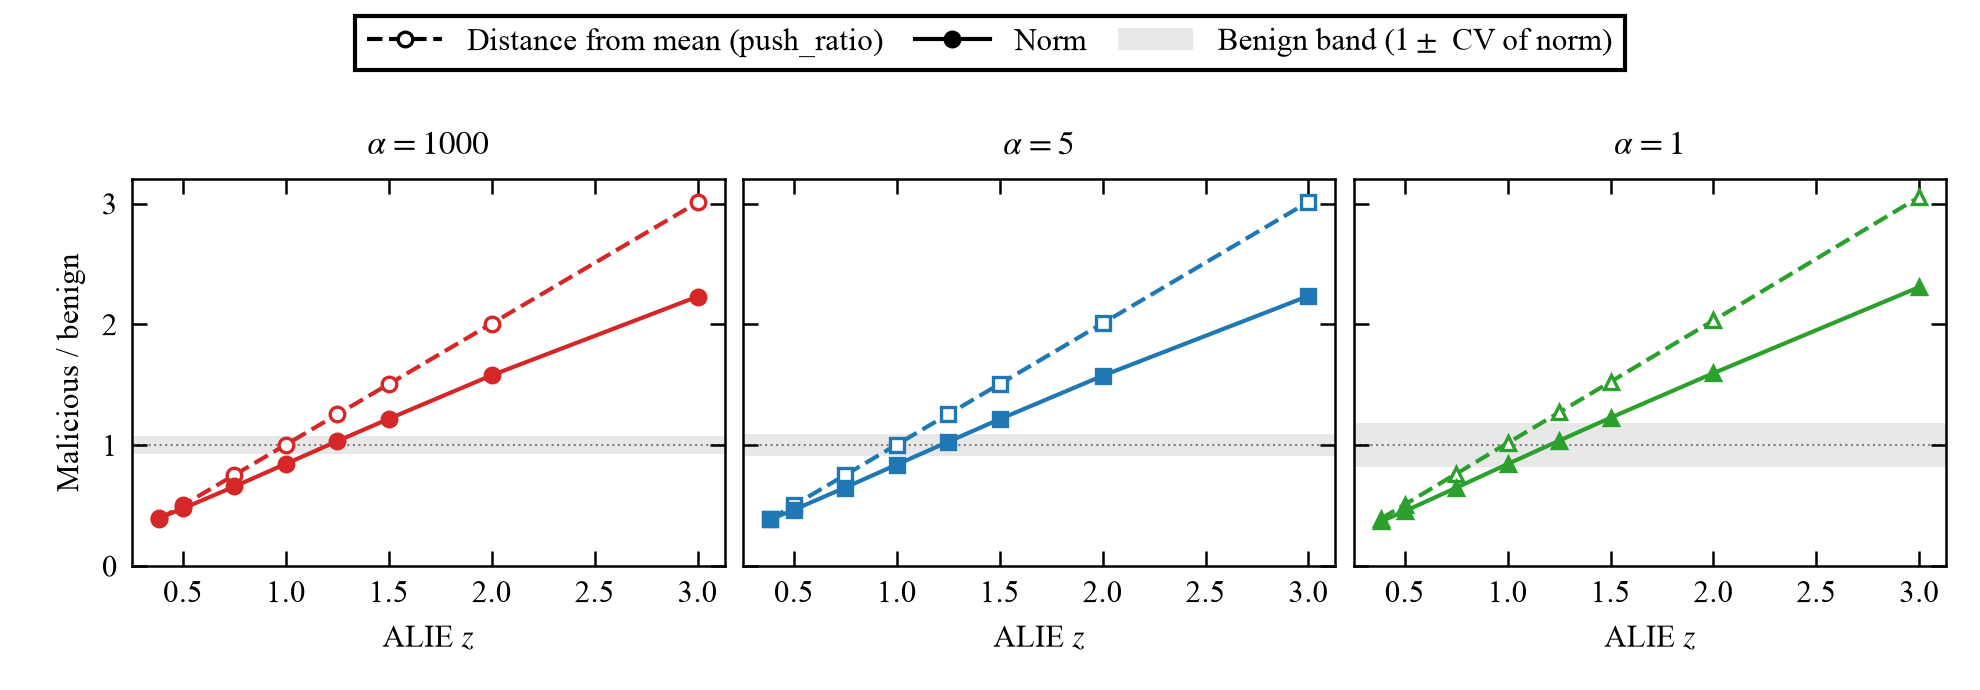
\includegraphics[width=0.85\textwidth]{fig/alie_shell_by_z_v3.png}
\caption{ALIEの $z$ と, 悪性更新の正常更新に対する比（第46--50ラウンド, 10試行の平均）. 破線（白抜きの印）は平均からの距離の比（\PushRatio{}）, 実線（塗りつぶしの印）はノルムの比. 灰色の帯は $1 \pm$ 正常更新のノルムの変動係数であり, 正常更新の殻の厚みの目安を表す. 点線は比 $1$}
\label{fig:alie-shell}
\end{figure*}

$z$ を大きくすると, 悪性更新は殻に近づき, $z$ がさらに大きくなると殻の外に出る（図\ref{fig:alie-shell}）. そのため, 距離やノルムに基づく検知が最も困難になるのは, 悪性更新が殻の上に来る付近である. D1のAUCは $z=1$--$1.5$ で低下し, 全 $\alpha$ で $z=1.25$ において最小（$0.09$--$0.16$）となったのち, $z \ge 2$ で再び $0.99$ 以上となった. 最小となる $z$ が $1$ ではなく $1.25$ であったのは, D1が平均からの距離ではなく原点からの長さであるノルムを用いるためである. 図\ref{fig:alie-shell}に示すように, 平均からの距離が正常更新と揃うのは $\PushRatio=1$, すなわち $z \approx 1$ であるのに対し, ノルムが揃うのは $z=1.25$ 付近であった（ノルムの比は $z=1$ で $0.84$--$0.85$, $z=1.25$ で $1.03$--$1.04$）. また, Non-IIDが強い $\alpha=1$ では, 正常更新のノルムのばらつきが大きく殻が厚いため, ノルムの比が殻の厚みの範囲に収まる $z$ の範囲が広く, D1のAUCが低下する $z$ の範囲も広かった（$z=1$ で $0.47$, $z=1.5$ で $0.72$）.

なお, 悪性更新が平均に近いという性質は, ALIEの設計に沿ったものである. 原論文は, 平均との差を小さくすることでKrumが計算するユークリッド距離を縮め, 悪性更新を選択させることを狙っている\cite{baruch2019little}（\ref{sec:attacks}節）. すなわち, ALIEが回避の対象とするのは, 外れた値を除外するTrimmed Meanや, 距離の近い更新を選ぶKrumであり, 平均に近すぎる更新を異常とみなす検知は想定されていない. したがって, $z<1$ のALIEが検知されたことは, ALIEが原論文の意図どおりに機能しなかったことを意味するのではなく, 原論文が想定していない種類の検知を適用した結果である.

以上より, 第三の問いに対しては次のようにいえる. 悪性更新を正常更新の平均に近づけることは, 検知を回避する手段にはならない. $\PushRatio=1$ は, それを下回ると検知が破綻する境界ではなく, 悪性更新が正常更新の殻の上に来て, 距離やノルムに基づく検知から最も隠れやすくなる点の近くである. その付近で検知が破綻するかどうかは, 検知器の性質と正常更新の分布によって異なった. D1はノルムが揃う $z=1.25$ 付近でのみ見分けられなくなり, その範囲はNon-IIDが強いほど広かった. 一方, D2は $z \le 1.5$ で, D4は $z$ が小さい範囲で悪性更新を最も正常らしいと判定しており, 破綻する $z$ は検知器ごとに異なった（\ref{sec:disc-detectors}節）.

\subsection{中心仮説の評価}
\label{sec:disc-hyp}

中心仮説は, (1) Non-IIDは正常更新のばらつき \Spread{} を増大させる, (2) 悪性更新が検知できるかどうかは \PushRatio{} でほぼ決まり, $1$ を下回ると検知性能が急落する, (3) したがってNon-IIDは検知性能を低下させる, という3つの主張からなる.

(1)の前提は, 学習の序盤には成り立ったが, 学習が進んだ段階ではほとんど成り立たなかった. \Spread{} は第1--5ラウンドではNon-IIDが強いほど約 $2.4$--$2.9$ 倍大きかったが, 第46--50ラウンドでは $1.00$--$1.08$ 倍にとどまった（\ref{sec:disc-noniid}節）.

(2)の中核は支持されなかった. 第一に, 符号反転では \PushRatio{} とAUCの順位相関は全体で $-0.32$--$-0.02$ であり, 仮説が予測する正の相関は見られなかった（表\ref{tab:corr}）. また, 符号反転の \PushRatio{} は全ラウンドを通じて $1$ を下回らなかったため（図\ref{fig:pushratio}）, 「$1$ を下回ると急落する」という予測は符号反転では検証できなかった. 第二に, ALIEで $\PushRatio<1$ に対応する $z<1$ の領域で検知性能は急落せず, D1ではむしろ高かった（\ref{sec:disc-rq3}節）. 第三に, ALIEの $z=0.75$ では \PushRatio{} がいずれの $\alpha$ でも約 $0.75$ であるにもかかわらず, D4のAUCは $\alpha$ によって $0.16$ から $1.00$ まで変化した（\ref{sec:disc-noniid}節）.

さらに, 符号反転の \PushRatio{} は, 学習の序盤には仮説の想定どおりNon-IIDが強いほど小さかった（第1--5ラウンドで $8.62$, $2.85$, $1.96$. 表\ref{tab:seg-push}）が, 学習の終盤には逆にNon-IIDが強いほど大きくなった（第46--50ラウンドで $1.58$, $2.03$, $2.55$. 表\ref{tab:pushratio}）. この逆転は, 分母の \Spread{} の差が縮む一方で, 分子の \Push{} がNon-IIDほど大きくなったことによる. \ref{sec:disc-detectors}節で述べたとおり, 悪性クライアントの更新は反転して集約されるため, グローバルモデルは悪性クライアントのデータに適合しにくくなり, 悪性クライアントのローカル学習での更新が大きくなる. その増え方はNon-IIDが強いほど大きく, 第46--50ラウンドにおける悪性更新のノルムの正常更新に対する比は $1.30$, $1.65$, $2.18$ であった（表\ref{tab:signflip-norm}）. すなわち, 終盤の \PushRatio{} の大小は, 中心仮説が想定した正常更新のばらつきではなく, 攻撃が学習を通じて悪性更新に与えた影響によって決まっていた.

(3)の帰結は, 検知性能が低下したという点では観測されたが, その理由は仮説の想定と異なった. Non-IIDによって検知性能が低下したのは, 符号反転に対するD1・D4と, ALIEに対するD2・D4であり, その低下と対応していたのは \Spread{} の大きさではなく, ばらつきの配分であった（\ref{sec:disc-noniid}節）.

仮説が外れた原因は, 主に2つあると考えられる. 第一に, 中心仮説は, 正常更新が平均の周りを埋めるという低次元の直感に基づいていた. 実際には, 高次元の正常更新は平均からほぼ一定の距離の殻の上に並ぶため, 平均に近い悪性更新は紛れずにむしろ目立った（\ref{sec:disc-rq3}節）. 第二に, \PushRatio{} は「正常更新の平均からの距離」という1つの量で悪性更新の位置をまとめたものであるが, 検知器はそれぞれ異なる量を見て, 異なる向きの外れを異常とみなす（\ref{sec:disc-detectors}節）. そのため, 同じ \PushRatio{} であっても, 検知器が見る量の上で悪性更新が正常更新の分布のどこに位置するかによって, 検知できるかどうかは異なった.

以上より, 中心仮説のうち, Non-IIDが検知性能を低下させるという帰結は観測されたが, 検知可能性が \PushRatio{} でほぼ決まるという中核と, その理由としての \Spread{} の増大は支持されなかった. 検知可能性を説明するには, 悪性更新と正常更新の平均との距離という1つの量ではなく, 検知器が見る量の上での悪性更新の位置と, 正常更新の分布の形を考慮する必要がある.

\subsection{妥当性への脅威と今後の課題}
\label{sec:disc-threats}

本研究の結果には次の制約がある.

まず, 本章の説明のいくつかは, 必要な量を記録していないため直接には確かめていない. 符号反転で悪性更新が大きくなる仕組み（\ref{sec:disc-detectors}節, \ref{sec:disc-hyp}節）はクライアントごとのローカル学習の損失を, ALIEでD2が逆転する説明（\ref{sec:disc-detectors}節）は参照方向 $r$ と正常更新のずれ $e_i$ を, 符号反転でD4が低下する説明（\ref{sec:disc-detectors}節）は第1主成分への射影の値を記録すれば確かめられる. なお, \ref{sec:disc-noniid}節の見積もりと\ref{sec:disc-rq3}節の殻による説明は, 結果を見たあとに整理したものである. ALIEでは悪性クライアント4台が同一のベクトルを送るため, D3の検知性能はこの性質に依存している可能性があり, 悪性更新にばらつきを持たせた場合に同じ結果が得られるかは確かめていない.

また, 表\ref{tab:corr}の順位相関は, 同じ実行の連続するラウンドをそれぞれ1点として数えている. 各ラウンドのモデルは前のラウンドの結果を引き継ぐため, 連続するラウンドの値は互いに似ており, 独立ではない. そのため, 点の数に比べて独立な情報は少なく, 本研究では有意性の検定を行わず, 相関の大きさを傾向の目安として扱った.

さらに, 実験の条件は限られている. データセットはMNISTのみであり, クライアント数は20, 学習データは $60{,}000$ 件のうち $30{,}000$ 件のみを用いた. Non-IIDはデータ数を揃えたラベルの偏りのみで与えており, 特徴の偏りやデータ数の偏りを含むNon-IIDで同じ結果が得られるかは分からない. 悪性の割合は $0.2$ のみであり, $\alpha$ は3水準, $z$ は8水準にとどまる. $\alpha=1$ の学習は50ラウンドで収束しておらず（\ref{sec:res-acc}節）, $\alpha=1$ の第46--50ラウンドの検知性能は学習が進みきる前の段階のものである.

加えて, 本研究は, 攻撃者が正常クライアントの更新を参照できるfull knowledgeを仮定した（第\ref{sec:threat}章）. 攻撃者が自身のデータから $\mu$ と $\sigma$ を推定するしかない場合には, 悪性更新の位置がずれるため, 結果が変わる可能性がある.

最後に, ALIEは, $\alpha \ge 5$ では $z=3$ でもグローバルモデルの精度をほとんど低下させず, $\alpha=1$ でも $z \le 1.5$ では低下が2ポイント以内であった（表\ref{tab:acc}）. ALIEは本来, Trimmed MeanやKrumなどのRobust Aggregationから隠れることを狙った攻撃であり, FedAvgはその対象ではない（\ref{sec:attacks}節）. したがって, 本研究の結果の多くは, FedAvgのもとで精度にほとんど害を与えない摂動が更新ベクトルのレベルで検知できるかを評価したものである. なお, 検知できることは防御できることと同じではなく, 検知した更新を集約から除いた場合に精度の低下を防げるかは評価していない.

今後の課題として, 次のものが挙げられる. 第一に, クライアントごとの損失や参照方向, 射影の値を記録し, 本章の解釈を直接確かめること. 第二に, 悪性更新にばらつきを持たせたALIEや, partial knowledgeの攻撃者を評価すること. 第三に, 特徴の偏りを含むFEMNISTなどのデータセットや, データ数の偏りを含むNon-IID, 異なる悪性の割合, より細かい $\alpha$ と $z$ の水準で評価すること. 第四に, ラウンド数を増やし, 学習が収束した段階での検知性能を確かめること. 第五に, 検知とRobust Aggregationを組み合わせ, 検知が精度の低下をどこまで防げるかを評価すること. これらを通じて, 本研究で示した検知可能性の説明が, より一般的な条件のもとでも成り立つかを確かめる必要がある.

% =========================================================
\section{おわりに}
\label{sec:conclusion}

本研究では, Federated Learning（FL）における悪性更新の検知を, データ分布の不均一性（Non-IID度）と攻撃のステルス性の2つの観点から評価した. Flowerを用いてFLを実装し, 符号反転攻撃とALIEに対して, 4種類の検知器が学習の途中で悪性更新をどの程度検知できるかを, ROC-AUCを用いて調べた. Non-IID度は $\alpha=1000,\,5,\,1$ の3水準, ALIEの係数 $z$ は $0.385$ から $3$ までの8水準とし, 各条件10試行, 計300回の実行を行った.

その結果, 検知器によって検知できる攻撃に差があることが分かった. 特に, 参照方向へのコサイン距離を用いる検知器（D2）は, $z \le 1.5$ のALIEに対して悪性更新を最も正常らしいと判定した. 検知できるかどうかは, 悪性更新が検知器の見る量の上でどこに位置し, 検知器がどの向きの外れを異常とみなすかによって決まっていた. また, Non-IIDは検知性能を低下させたが, その原因は正常更新のばらつきの大きさ \Spread{} ではなく, ばらつきの配分, すなわち正常更新のノルムのばらつき, 全クライアントに共通する成分と各クライアントのずれの大きさの比, およびばらつきが特定の方向に集中する度合いであった. さらに, 高次元の正常更新は平均からほぼ一定の距離の殻の上に並ぶため, 平均に近い悪性更新は紛れずにむしろ目立った. 距離やノルムに基づく検知では, 悪性更新が殻の上に来る $z=1$--$1.5$ 付近で検知性能が低下し, それより内側や外側では検知できた.

中心仮説は支持されなかった. 符号反転では \PushRatio{} とAUCに正の相関がなく, ALIEでは \PushRatio{} を $1$ 未満にしても検知性能は急落せず, 同じ \PushRatio{} でもD4のAUCはNon-IID度によって大きく異なった.

なお, 本研究のALIEの多くはFedAvgのもとで精度をほとんど低下させておらず, 本研究の結果は主に検知性能に関するものである. 今後の課題として, 本研究ではラベルの偏りだけという単純化したNon-IIDで評価したこと, MNISTと20台のクライアントという小規模な設定であったこと, $\alpha=1$ では学習が収束する前に50ラウンドが終わったことから, より現実に近いNon-IIDと大きな規模, 十分なラウンド数での評価が挙げられる. また, 複数の検知器を組み合わせた場合の検知性能の評価も今後の課題である.

% =========================================================
\clearpage
\begin{thebibliography}{99}

\bibitem{mammen2021fl}
Priyanka Mary Mammen,
``Federated Learning: Opportunities and Challenges,''
arXiv preprint arXiv:2101.05428, 2021.

\bibitem{li2019fl}
Tian Li, Anit Kumar Sahu, Ameet Talwalkar, Virginia Smith,
``Federated Learning: Challenges, Methods, and Future Directions,''
arXiv preprint arXiv:1908.07873, 2019.

\bibitem{ma2020privacy}
Chuan Ma, Jun Li, Ming Ding, Howard H. Yang, Feng Shu, Tony Q. S. Quek, H. Vincent Poor,
``On Safeguarding Privacy and Security in the Framework of Federated Learning,''
IEEE Network, vol.~34, no.~4, pp.~242--248, 2020.

\bibitem{sagar2023survey}
Subhash Sagar, Chang-Tsun Li, Seng W. Loke, Jinho Choi,
``Poisoning Attacks and Defenses in Federated Learning: A Survey,''
arXiv preprint arXiv:2301.05795, 2023.

\bibitem{fang2020local}
Minghong Fang, Xiaoyu Cao, Jinyuan Jia, Neil Zhenqiang Gong,
``Local Model Poisoning Attacks to Byzantine-Robust Federated Learning,''
Proceedings of the 29th USENIX Security Symposium (USENIX Security 2020),
pp.~1605--1622, 2020.

\bibitem{baruch2019little}
Gilad Baruch, Moran Baruch, Yoav Goldberg,
``A Little Is Enough: Circumventing Defenses For Distributed Learning,''
Advances in Neural Information Processing Systems (NeurIPS), 2019.

\bibitem{mcmahan2017fedavg}
H.~Brendan McMahan, Eider Moore, Daniel Ramage, Seth Hampson, Blaise Aguera y Arcas,
``Communication-Efficient Learning of Deep Networks from Decentralized Data,''
Proceedings of the 20th International Conference on Artificial Intelligence and Statistics (AISTATS),
pp.~1273--1282, 2017.

\bibitem{li2022federated}
Qinbin Li, Yiqun Diao, Quan Chen, Bingsheng He,
``Federated Learning on Non-IID Data Silos: An Experimental Study,''
Proceedings of the 38th IEEE International Conference on Data Engineering (ICDE), 2022.

\bibitem{xie2020dba}
Chulin Xie, Keli Huang, Pin-Yu Chen, Bo Li,
``DBA: Distributed Backdoor Attacks against Federated Learning,''
International Conference on Learning Representations (ICLR), 2020.

\bibitem{nguyen2022flame}
Thien Duc Nguyen et al.,
``FLAME: Taming Backdoors in Federated Learning,''
31st USENIX Security Symposium (USENIX Security 2022), pp.~1415--1432, 2022.

\bibitem{bagdasaryan2020model}
Eugene Bagdasaryan, Andreas Veit, Yiqing Hua, Deborah Estrin, Vitaly Shmatikov,
``How To Backdoor Federated Learning,''
Proceedings of the 23rd International Conference on Artificial Intelligence and Statistics (AISTATS),
pp.~2938--2948, 2020.

\bibitem{shejwalkar2021manipulating}
Virat Shejwalkar, Amir Houmansadr,
``Manipulating the Byzantine: Optimizing Model Poisoning Attacks and Defenses for Federated Learning,''
Network and Distributed System Security Symposium (NDSS), 2021.

\bibitem{yin2018byzantine}
Dong Yin, Yudong Chen, Kannan Ramchandran, Peter Bartlett,
``Byzantine-Robust Distributed Learning: Towards Optimal Statistical Rates,''
Proceedings of the 35th International Conference on Machine Learning (ICML), 2018.

\bibitem{blanchard2017krum}
Peva Blanchard, El Mahdi El Mhamdi, Rachid Guerraoui, Julien Stainer,
``Machine Learning with Adversaries: Byzantine Tolerant Gradient Descent,''
Advances in Neural Information Processing Systems (NeurIPS), 2017.

\bibitem{elmhamdi2018hidden}
El Mahdi El Mhamdi, Rachid Guerraoui, S\'ebastien Rouault,
``The Hidden Vulnerability of Distributed Learning in Byzantium,''
Proceedings of the 35th International Conference on Machine Learning (ICML), 2018.

\bibitem{shen2016auror}
Shiqi Shen, Shruti Tople, Prateek Saxena,
``Auror: Defending Against Poisoning Attacks in Collaborative Deep Learning Systems,''
Proceedings of the 32nd Annual Conference on Computer Security Applications (ACSAC), 2016.

\bibitem{tran2018spectral}
Brandon Tran, Jerry Li, Aleksander Madry,
``Spectral Signatures in Backdoor Attacks,''
Advances in Neural Information Processing Systems (NeurIPS), 2018.

\bibitem{fawcett2006roc}
Tom Fawcett,
``An Introduction to ROC Analysis,''
Pattern Recognition Letters, vol.~27, no.~8, pp.~861--874, 2006.

\bibitem{hanley1982meaning}
James A. Hanley, Barbara J. McNeil,
``The Meaning and Use of the Area under a Receiver Operating Characteristic (ROC) Curve,''
Radiology, vol.~143, no.~1, pp.~29--36, 1982.

\bibitem{hsu2019measuring}
Tzu-Ming Harry Hsu, Hang Qi, Matthew Brown,
``Measuring the Effects of Non-Identical Data Distribution for Federated Visual Classification,''
arXiv preprint arXiv:1909.06335, 2019.

\bibitem{li2023experimental}
Shenghui Li, Edith C.-H. Ngai, Thiemo Voigt,
``An Experimental Study of Byzantine-Robust Aggregation Schemes in Federated Learning,''
arXiv preprint arXiv:2302.07173, 2023.

\bibitem{wang2023trust}
Zhilin Wang, Qin Hu, Xukai Zou,
``Can We Trust the Similarity Measurement in Federated Learning?,''
arXiv preprint arXiv:2311.03369, 2023.

\bibitem{cao2021fltrust}
Xiaoyu Cao, Minghong Fang, Jia Liu, Neil Zhenqiang Gong,
``FLTrust: Byzantine-robust Federated Learning via Trust Bootstrapping,''
Network and Distributed System Security Symposium (NDSS), 2021.

\bibitem{shejwalkar2022back}
Virat Shejwalkar, Amir Houmansadr, Peter Kairouz, Daniel Ramage,
``Back to the Drawing Board: A Critical Evaluation of Poisoning Attacks on Production Federated Learning,''
IEEE Symposium on Security and Privacy (S\&P), 2022.

\bibitem{beutel2020flower}
Daniel J. Beutel, Taner Topal, Akhil Mathur, Xinchi Qiu, Javier Fernandez-Marques, Yan Gao, Lorenzo Sani, Kwing Hei Li, Titouan Parcollet, Pedro Porto Buarque de Gusm\~{a}o, Nicholas D. Lane,
``Flower: A Friendly Federated Learning Research Framework,''
arXiv preprint arXiv:2007.14390, 2020.

\end{thebibliography}

% =========================================================
\onecolumn
\appendix
\section{AUCのラウンド推移（全水準）}
\label{sec:appendix-rounds}

図\ref{fig:auc-round-all}に, ALIEの8水準すべてと符号反転について, 検知器ごとのAUCのラウンド推移を示す. 図の見方は図\ref{fig:auc-round}と同じである.

\begin{figure}[H]
\centering
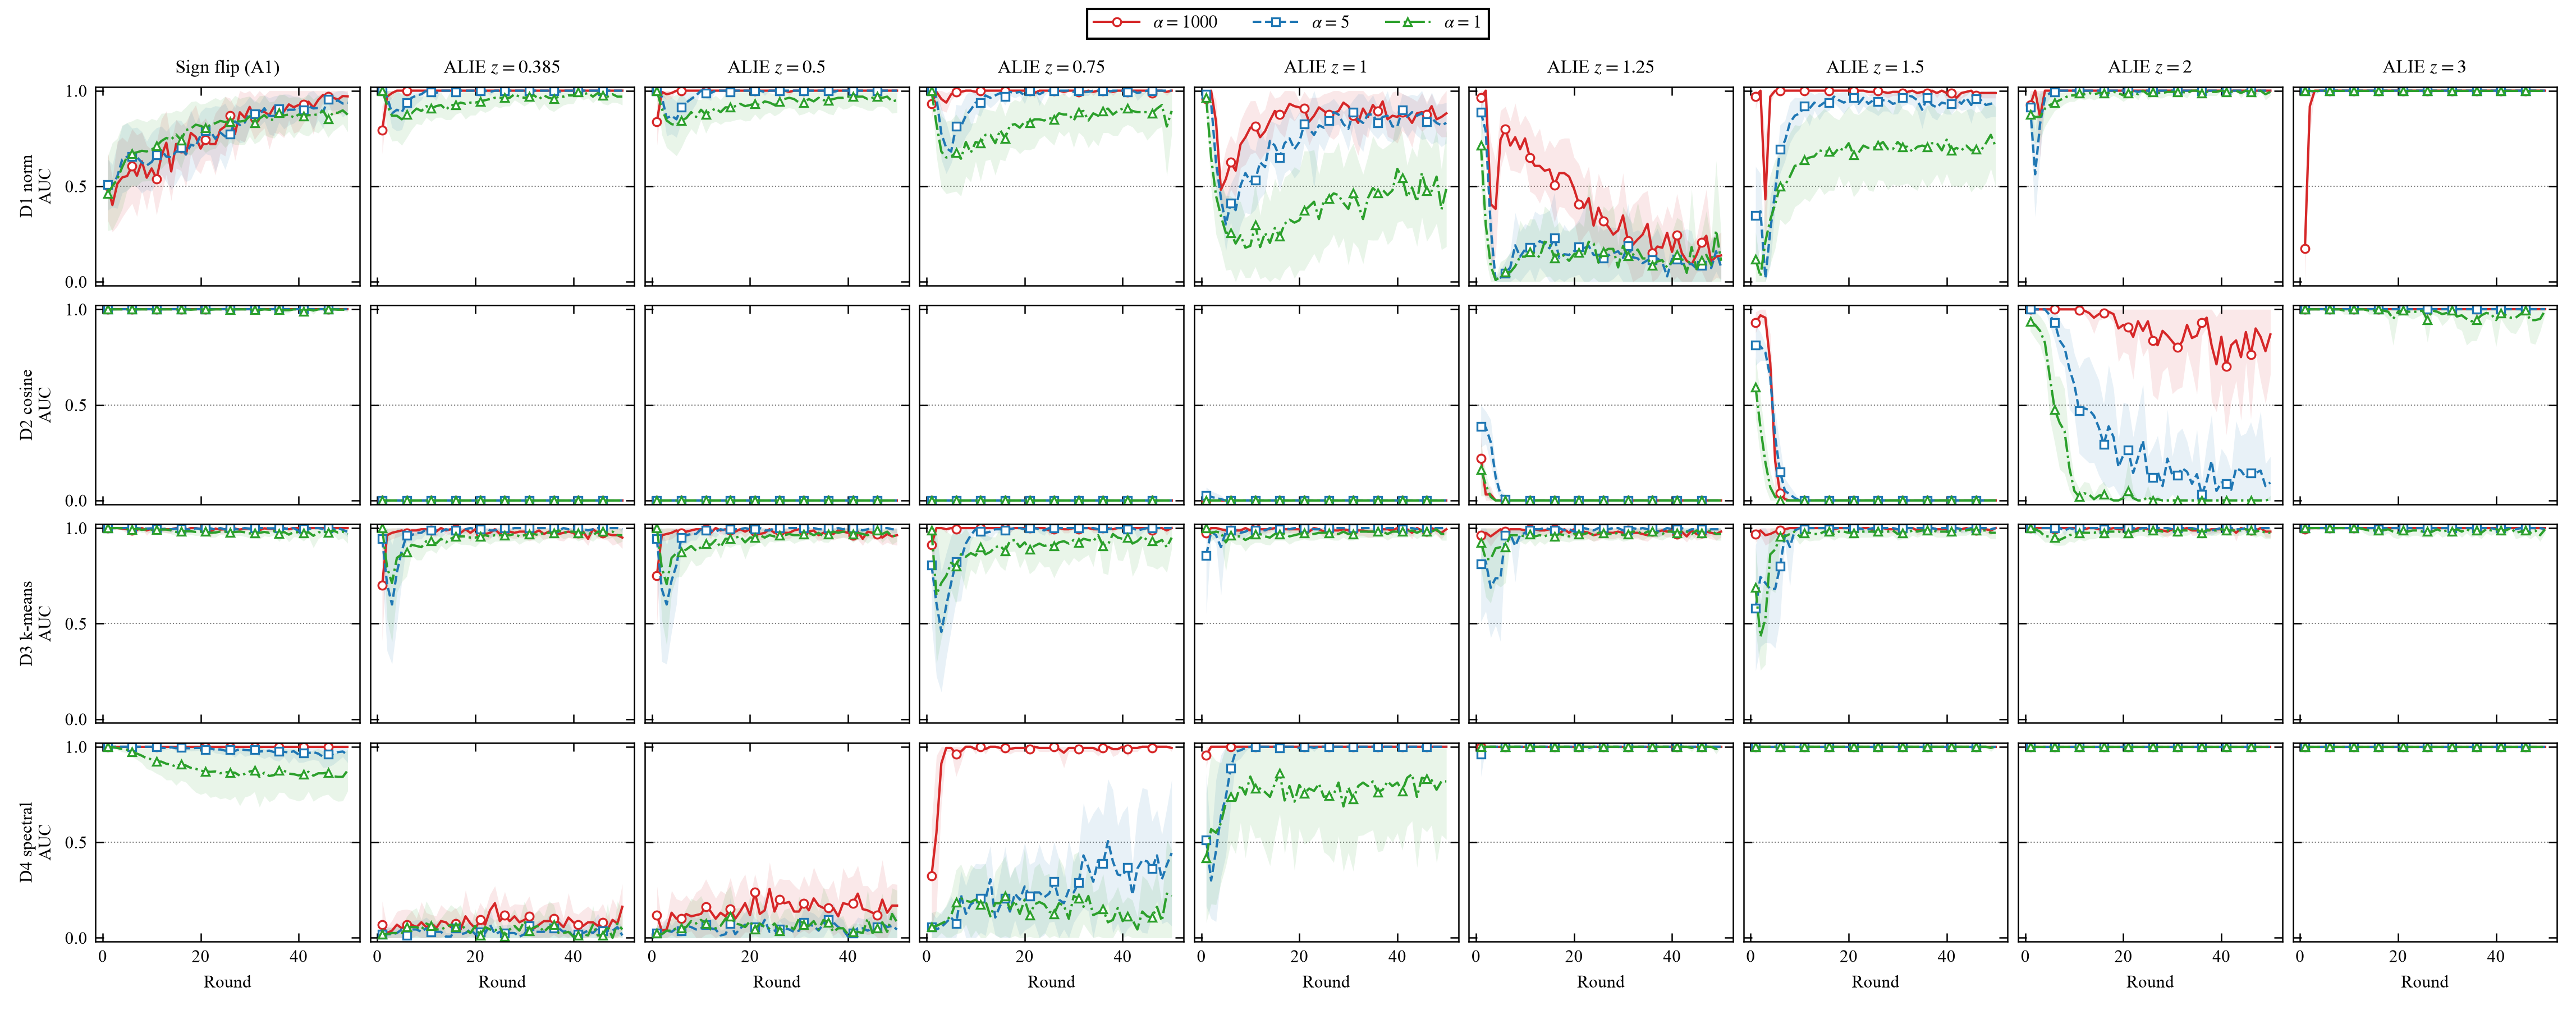
\includegraphics[width=\textwidth]{fig/detection_auc_by_round_v3.png}
\caption{AUCのラウンド推移（全水準）. 行は検知器D1--D4, 列は攻撃（符号反転と, ALIEの $z=0.385,\,0.5,\,0.75,\,1,\,1.25,\,1.5,\,2,\,3$）. 線は試行間の平均, 帯は$\pm$標準偏差. 赤実線○: $\alpha=1000$, 青破線□: $\alpha=5$, 緑一点鎖線△: $\alpha=1$. 点線は $\mathrm{AUC}=0.5$}
\label{fig:auc-round-all}
\end{figure}

\section{ラウンドの区間ごとのAUC}
\label{sec:appendix-segments}

表\ref{tab:seg-d1}--\ref{tab:seg-d4}に, 検知器ごとに, ラウンドを第1--5, 6--15, 16--30, 31--50ラウンドの4区間に分けて平均したAUCを示す. 各値は, 試行ごとに区間内のラウンドのAUCを平均したうえで, 10試行について平均したものである. \ref{sec:res-rounds}節で述べる区間ごとの値は, これらの表による.

\begin{table}[H]
\centering
\caption{ラウンドの区間ごとのAUC: D1（ノルム偏差）（区間内のラウンドを試行ごとに平均したうえでの10試行の平均）}
\label{tab:seg-d1}
\footnotesize
\tabcolsep=3.2pt
\begin{tabular}{@{}l@{\hspace{5pt}}cccc@{\hspace{8pt}}cccc@{\hspace{8pt}}cccc@{}}
\toprule
 & \multicolumn{4}{c}{$\alpha=1000$} & \multicolumn{4}{c}{$\alpha=5$} & \multicolumn{4}{c}{$\alpha=1$} \\
\cmidrule(lr){2-5}\cmidrule(lr){6-9}\cmidrule(l){10-13}
攻撃 & 1--5 & 6--15 & 16--30 & 31--50 & 1--5 & 6--15 & 16--30 & 31--50 & 1--5 & 6--15 & 16--30 & 31--50 \\
\midrule
A1 符号反転 & 0.50 & 0.61 & 0.78 & 0.93 & 0.57 & 0.65 & 0.77 & 0.91 & 0.55 & 0.71 & 0.82 & 0.87 \\
\midrule
A2 $z{=}0.385$ & 0.95 & 1.00 & 1.00 & 1.00 & 0.93 & 0.98 & 1.00 & 1.00 & 0.90 & 0.91 & 0.95 & 0.97 \\
A2 $z{=}0.5$ & 0.96 & 1.00 & 1.00 & 1.00 & 0.91 & 0.98 & 1.00 & 1.00 & 0.88 & 0.88 & 0.93 & 0.96 \\
A2 $z{=}0.75$ & 0.96 & 1.00 & 1.00 & 1.00 & 0.82 & 0.92 & 0.99 & 1.00 & 0.76 & 0.72 & 0.84 & 0.89 \\
A2 $z{=}1$ & 0.76 & 0.76 & 0.90 & 0.88 & 0.66 & 0.56 & 0.79 & 0.85 & 0.53 & 0.23 & 0.37 & 0.47 \\
A2 $z{=}1.25$ & 0.70 & 0.67 & 0.40 & 0.18 & 0.40 & 0.16 & 0.15 & 0.10 & 0.23 & 0.13 & 0.15 & 0.12 \\
A2 $z{=}1.5$ & 0.87 & 1.00 & 1.00 & 0.99 & 0.30 & 0.86 & 0.95 & 0.94 & 0.22 & 0.61 & 0.70 & 0.71 \\
A2 $z{=}2$ & 0.96 & 1.00 & 1.00 & 1.00 & 0.85 & 1.00 & 1.00 & 1.00 & 0.89 & 0.97 & 0.99 & 0.99 \\
A2 $z{=}3$ & 0.82 & 1.00 & 1.00 & 1.00 & 1.00 & 1.00 & 1.00 & 1.00 & 1.00 & 1.00 & 1.00 & 1.00 \\
\bottomrule
\end{tabular}
\end{table}

\begin{table}[H]
\centering
\caption{ラウンドの区間ごとのAUC: D2（コサイン距離）（区間内のラウンドを試行ごとに平均したうえでの10試行の平均）}
\label{tab:seg-d2}
\footnotesize
\tabcolsep=3.2pt
\begin{tabular}{@{}l@{\hspace{5pt}}cccc@{\hspace{8pt}}cccc@{\hspace{8pt}}cccc@{}}
\toprule
 & \multicolumn{4}{c}{$\alpha=1000$} & \multicolumn{4}{c}{$\alpha=5$} & \multicolumn{4}{c}{$\alpha=1$} \\
\cmidrule(lr){2-5}\cmidrule(lr){6-9}\cmidrule(l){10-13}
攻撃 & 1--5 & 6--15 & 16--30 & 31--50 & 1--5 & 6--15 & 16--30 & 31--50 & 1--5 & 6--15 & 16--30 & 31--50 \\
\midrule
A1 符号反転 & 1.00 & 1.00 & 1.00 & 1.00 & 1.00 & 1.00 & 1.00 & 1.00 & 1.00 & 1.00 & 1.00 & 1.00 \\
\midrule
A2 $z{=}0.385$ & 0.00 & 0.00 & 0.00 & 0.00 & 0.00 & 0.00 & 0.00 & 0.00 & 0.00 & 0.00 & 0.00 & 0.00 \\
A2 $z{=}0.5$ & 0.00 & 0.00 & 0.00 & 0.00 & 0.00 & 0.00 & 0.00 & 0.00 & 0.00 & 0.00 & 0.00 & 0.00 \\
A2 $z{=}0.75$ & 0.00 & 0.00 & 0.00 & 0.00 & 0.00 & 0.00 & 0.00 & 0.00 & 0.00 & 0.00 & 0.00 & 0.00 \\
A2 $z{=}1$ & 0.00 & 0.00 & 0.00 & 0.00 & 0.01 & 0.00 & 0.00 & 0.00 & 0.00 & 0.00 & 0.00 & 0.00 \\
A2 $z{=}1.25$ & 0.06 & 0.00 & 0.00 & 0.00 & 0.25 & 0.00 & 0.00 & 0.00 & 0.05 & 0.00 & 0.00 & 0.00 \\
A2 $z{=}1.5$ & 0.76 & 0.00 & 0.00 & 0.00 & 0.67 & 0.02 & 0.00 & 0.00 & 0.25 & 0.00 & 0.00 & 0.00 \\
A2 $z{=}2$ & 1.00 & 0.99 & 0.90 & 0.83 & 0.99 & 0.61 & 0.21 & 0.12 & 0.84 & 0.16 & 0.01 & 0.00 \\
A2 $z{=}3$ & 1.00 & 1.00 & 1.00 & 1.00 & 1.00 & 1.00 & 1.00 & 1.00 & 1.00 & 1.00 & 0.98 & 0.96 \\
\bottomrule
\end{tabular}
\end{table}

\begin{table}[H]
\centering
\caption{ラウンドの区間ごとのAUC: D3（2クラスタリング）（区間内のラウンドを試行ごとに平均したうえでの10試行の平均）}
\label{tab:seg-d3}
\footnotesize
\tabcolsep=3.2pt
\begin{tabular}{@{}l@{\hspace{5pt}}cccc@{\hspace{8pt}}cccc@{\hspace{8pt}}cccc@{}}
\toprule
 & \multicolumn{4}{c}{$\alpha=1000$} & \multicolumn{4}{c}{$\alpha=5$} & \multicolumn{4}{c}{$\alpha=1$} \\
\cmidrule(lr){2-5}\cmidrule(lr){6-9}\cmidrule(l){10-13}
攻撃 & 1--5 & 6--15 & 16--30 & 31--50 & 1--5 & 6--15 & 16--30 & 31--50 & 1--5 & 6--15 & 16--30 & 31--50 \\
\midrule
A1 符号反転 & 1.00 & 0.99 & 1.00 & 1.00 & 1.00 & 1.00 & 1.00 & 1.00 & 1.00 & 0.99 & 0.98 & 0.98 \\
\midrule
A2 $z{=}0.385$ & 0.92 & 0.99 & 0.98 & 0.97 & 0.78 & 0.98 & 1.00 & 1.00 & 0.84 & 0.92 & 0.96 & 0.97 \\
A2 $z{=}0.5$ & 0.93 & 0.99 & 0.98 & 0.97 & 0.75 & 0.98 & 1.00 & 1.00 & 0.84 & 0.91 & 0.96 & 0.97 \\
A2 $z{=}0.75$ & 0.98 & 1.00 & 1.00 & 1.00 & 0.64 & 0.95 & 1.00 & 1.00 & 0.78 & 0.87 & 0.92 & 0.94 \\
A2 $z{=}1$ & 0.99 & 0.99 & 0.99 & 0.99 & 0.94 & 0.99 & 1.00 & 1.00 & 0.97 & 0.96 & 0.97 & 0.98 \\
A2 $z{=}1.25$ & 0.97 & 0.99 & 0.98 & 0.98 & 0.76 & 0.97 & 0.99 & 0.99 & 0.88 & 0.96 & 0.97 & 0.98 \\
A2 $z{=}1.5$ & 0.97 & 1.00 & 1.00 & 1.00 & 0.68 & 0.96 & 1.00 & 1.00 & 0.68 & 0.97 & 0.98 & 0.98 \\
A2 $z{=}2$ & 1.00 & 1.00 & 0.99 & 0.99 & 1.00 & 1.00 & 1.00 & 1.00 & 0.98 & 0.97 & 0.98 & 0.99 \\
A2 $z{=}3$ & 1.00 & 1.00 & 1.00 & 1.00 & 1.00 & 1.00 & 1.00 & 1.00 & 1.00 & 1.00 & 0.99 & 0.99 \\
\bottomrule
\end{tabular}
\end{table}

\begin{table}[H]
\centering
\caption{ラウンドの区間ごとのAUC: D4（スペクトル残差）（区間内のラウンドを試行ごとに平均したうえでの10試行の平均）}
\label{tab:seg-d4}
\footnotesize
\tabcolsep=3.2pt
\begin{tabular}{@{}l@{\hspace{5pt}}cccc@{\hspace{8pt}}cccc@{\hspace{8pt}}cccc@{}}
\toprule
 & \multicolumn{4}{c}{$\alpha=1000$} & \multicolumn{4}{c}{$\alpha=5$} & \multicolumn{4}{c}{$\alpha=1$} \\
\cmidrule(lr){2-5}\cmidrule(lr){6-9}\cmidrule(l){10-13}
攻撃 & 1--5 & 6--15 & 16--30 & 31--50 & 1--5 & 6--15 & 16--30 & 31--50 & 1--5 & 6--15 & 16--30 & 31--50 \\
\midrule
A1 符号反転 & 1.00 & 1.00 & 1.00 & 1.00 & 1.00 & 1.00 & 0.99 & 0.97 & 0.99 & 0.93 & 0.87 & 0.86 \\
\midrule
A2 $z{=}0.385$ & 0.05 & 0.07 & 0.10 & 0.08 & 0.03 & 0.03 & 0.03 & 0.04 & 0.02 & 0.06 & 0.05 & 0.04 \\
A2 $z{=}0.5$ & 0.09 & 0.12 & 0.16 & 0.16 & 0.03 & 0.04 & 0.05 & 0.06 & 0.03 & 0.07 & 0.07 & 0.06 \\
A2 $z{=}0.75$ & 0.76 & 0.99 & 0.99 & 0.99 & 0.07 & 0.18 & 0.22 & 0.37 & 0.08 & 0.18 & 0.16 & 0.14 \\
A2 $z{=}1$ & 0.99 & 1.00 & 1.00 & 1.00 & 0.53 & 0.98 & 1.00 & 1.00 & 0.57 & 0.77 & 0.77 & 0.80 \\
A2 $z{=}1.25$ & 1.00 & 1.00 & 1.00 & 1.00 & 0.99 & 1.00 & 1.00 & 1.00 & 1.00 & 1.00 & 1.00 & 1.00 \\
A2 $z{=}1.5$ & 1.00 & 1.00 & 1.00 & 1.00 & 1.00 & 1.00 & 1.00 & 1.00 & 1.00 & 1.00 & 1.00 & 1.00 \\
A2 $z{=}2$ & 1.00 & 1.00 & 1.00 & 1.00 & 1.00 & 1.00 & 1.00 & 1.00 & 1.00 & 1.00 & 1.00 & 1.00 \\
A2 $z{=}3$ & 1.00 & 1.00 & 1.00 & 1.00 & 1.00 & 1.00 & 1.00 & 1.00 & 1.00 & 1.00 & 1.00 & 1.00 \\
\bottomrule
\end{tabular}
\end{table}

\section{ラウンドの区間ごとの \PushRatio{}}
\label{sec:appendix-pushratio}

表\ref{tab:seg-push}に, ラウンドを第1--5, 6--15, 16--30, 31--50ラウンドの4区間に分けて平均した \PushRatio{} を示す. 各値は, 試行ごとに区間内のラウンドの値を平均したうえで, 10試行について平均したものである.

\begin{table}[H]
\centering
\caption{ラウンドの区間ごとの \PushRatio{}（区間内のラウンドを試行ごとに平均したうえでの10試行の平均）}
\label{tab:seg-push}
\footnotesize
\tabcolsep=3.2pt
\begin{tabular}{@{}l@{\hspace{5pt}}cccc@{\hspace{8pt}}cccc@{\hspace{8pt}}cccc@{}}
\toprule
 & \multicolumn{4}{c}{$\alpha=1000$} & \multicolumn{4}{c}{$\alpha=5$} & \multicolumn{4}{c}{$\alpha=1$} \\
\cmidrule(lr){2-5}\cmidrule(lr){6-9}\cmidrule(l){10-13}
攻撃 & 1--5 & 6--15 & 16--30 & 31--50 & 1--5 & 6--15 & 16--30 & 31--50 & 1--5 & 6--15 & 16--30 & 31--50 \\
\midrule
A1 符号反転 & 8.62 & 2.44 & 1.70 & 1.57 & 2.85 & 2.13 & 1.83 & 1.93 & 1.96 & 1.99 & 2.15 & 2.41 \\
\midrule
A2 $z{=}0.385$ & 0.39 & 0.39 & 0.39 & 0.39 & 0.39 & 0.39 & 0.39 & 0.39 & 0.39 & 0.39 & 0.39 & 0.39 \\
A2 $z{=}0.5$ & 0.50 & 0.50 & 0.50 & 0.50 & 0.50 & 0.50 & 0.50 & 0.50 & 0.51 & 0.51 & 0.51 & 0.51 \\
A2 $z{=}0.75$ & 0.75 & 0.75 & 0.75 & 0.75 & 0.76 & 0.75 & 0.75 & 0.75 & 0.76 & 0.77 & 0.76 & 0.76 \\
A2 $z{=}1$ & 1.00 & 1.00 & 1.00 & 1.00 & 1.01 & 1.01 & 1.00 & 1.00 & 1.01 & 1.02 & 1.02 & 1.01 \\
A2 $z{=}1.25$ & 1.25 & 1.25 & 1.25 & 1.25 & 1.26 & 1.26 & 1.25 & 1.25 & 1.26 & 1.28 & 1.27 & 1.27 \\
A2 $z{=}1.5$ & 1.50 & 1.50 & 1.50 & 1.50 & 1.51 & 1.51 & 1.51 & 1.51 & 1.52 & 1.53 & 1.53 & 1.52 \\
A2 $z{=}2$ & 2.01 & 2.00 & 2.00 & 2.01 & 2.02 & 2.01 & 2.01 & 2.01 & 2.02 & 2.04 & 2.03 & 2.03 \\
A2 $z{=}3$ & 3.01 & 3.00 & 3.01 & 3.01 & 3.03 & 3.02 & 3.01 & 3.01 & 3.03 & 3.06 & 3.06 & 3.05 \\
\bottomrule
\end{tabular}
\end{table}

\section{悪性値の座標ごとの順位と正規分布からの予想値}
\label{sec:appendix-rank}

表\ref{tab:rank}に, ALIEの各 $z$ について, 悪性値の座標ごとの順位の平均と $\Phi(-z)$ を示す.

\begin{table}[H]
\centering
\caption{ALIEにおける悪性値の座標ごとの順位の平均（第46--50ラウンド, 10試行の平均）と $\Phi(-z)$}
\label{tab:rank}
\begin{tabular}{@{}ccccc@{}}
\toprule
 & & \multicolumn{3}{c}{順位の平均} \\
\cmidrule(l){3-5}
$z$ & $\Phi(-z)$ & $\alpha=1000$ & $\alpha=5$ & $\alpha=1$ \\
\midrule
$0.385$ & $0.350$ & $0.339$ & $0.342$ & $0.350$ \\
$0.5$ & $0.309$ & $0.298$ & $0.301$ & $0.307$ \\
$0.75$ & $0.227$ & $0.224$ & $0.225$ & $0.229$ \\
$1$ & $0.159$ & $0.167$ & $0.167$ & $0.170$ \\
$1.25$ & $0.106$ & $0.124$ & $0.124$ & $0.130$ \\
$1.5$ & $0.067$ & $0.094$ & $0.096$ & $0.108$ \\
$2$ & $0.023$ & $0.064$ & $0.075$ & $0.103$ \\
$3$ & $0.001$ & $0.073$ & $0.110$ & $0.180$ \\
\bottomrule
\end{tabular}
\end{table}

\end{document}